\chapter{Hardware}

%sección 4.1
\section{Arquitecturas estudiadas}\label{arqEst}
Se plantearon varias alternativas como posible solución. A medida que se encontraron limitantes o que no se cumplían los requerimientos exigidos, se fueron descartando dichas opciones.

A continuación se describen algunas de las arquitecturas consideradas:

\begin{itemize}
\item[1 -] OpenPCD + lector de tarjetas de contacto + display + buzzer + leds
\bigskip

\begin{figure}[H]
\centering
  \begin{center}
  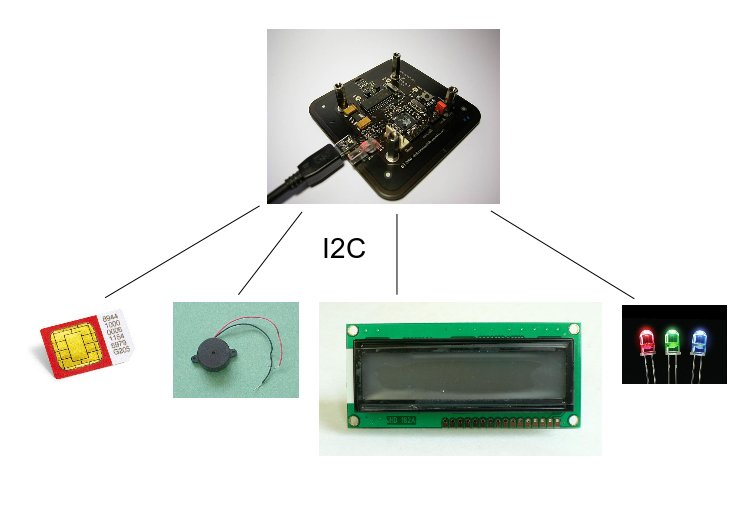
\includegraphics[scale=.4]{Imagenes/0.jpg} 
  \end{center}
  \caption{Solución considerada 1}\label{Fig:HW1} 
\end{figure}

\newpage
Al dispositivo OpenPCD, se conecta el resto del hardware a través de su único puerto de entrada/salida disponible que es de tipo I2C.

\bigskip
\item[2 -] SBC + OpenPCD + microcontrolador + lector de tarjetas de contacto + display + buzzer + leds
\bigskip

\begin{figure}[H]
\centering
  \begin{center}
  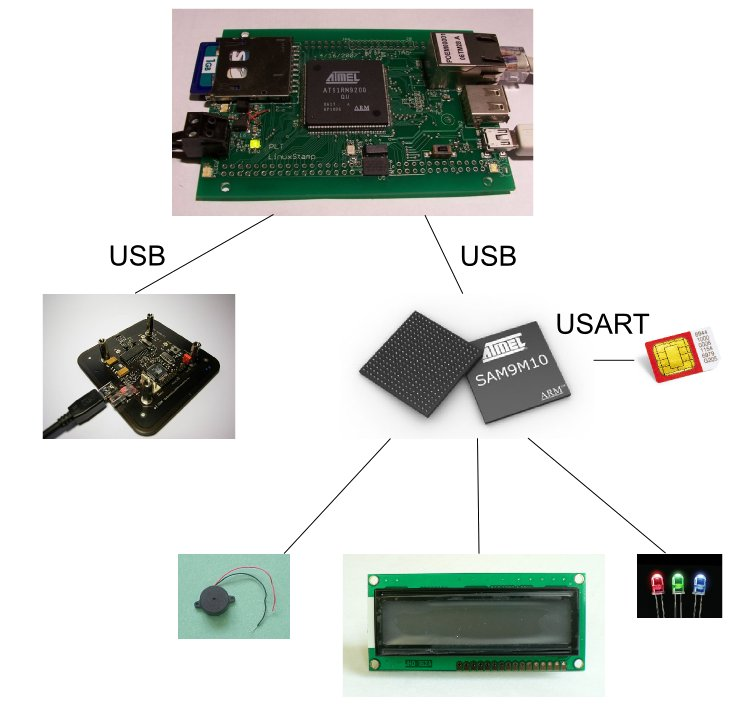
\includegraphics[scale=.3]{Imagenes/1.jpg} 
  \end{center}
  \caption{Solución considerada 2}\label{Fig:HW2} 
\end{figure}

Tanto el dispositivo OpenPCD como el microcontrolador se conectan directamente por USB a la SBC. El microcontrolador maneja el resto de los dispositivos (lector de tarjetas de contacto, display, buzzer y leds).

\bigskip
\item[3 -] SBC + OpenPCD + lector de tarjetas de contacto + display + buzzer + leds
\bigskip

\begin{figure}[H]
\centering
  \begin{center}
  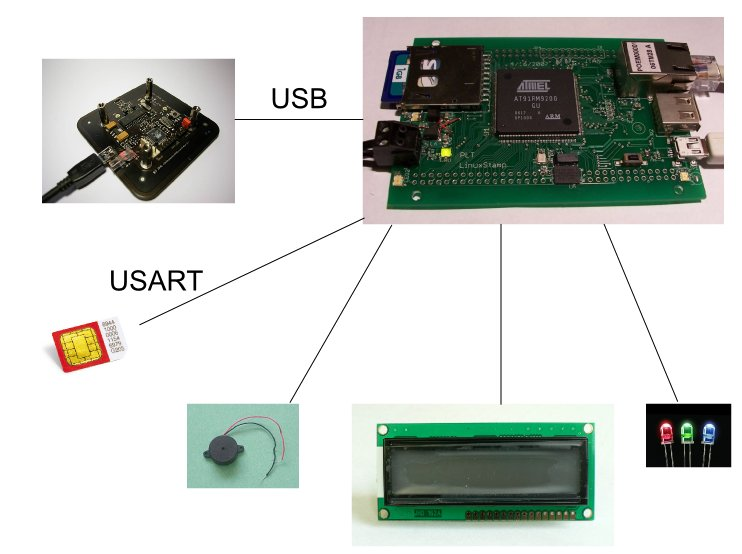
\includegraphics[scale=.25]{Imagenes/2.jpg} 
  \end{center}
  \caption{Solución considerada 3}\label{Fig:HW3} 
\end{figure}

El dispositivo OpenPCD se conecta por USB a la SBC. La SBC maneja los dispositivos (lector de tarjetas de contacto, display, buzzer y leds) a través de sus interfaces nativas.

\bigskip
\item[4 -] SBC + lector de tarjetas RFID + lector de tarjetas de contacto + display + buzzer + leds
\bigskip

\begin{figure}[H]
\centering
  \begin{center}
  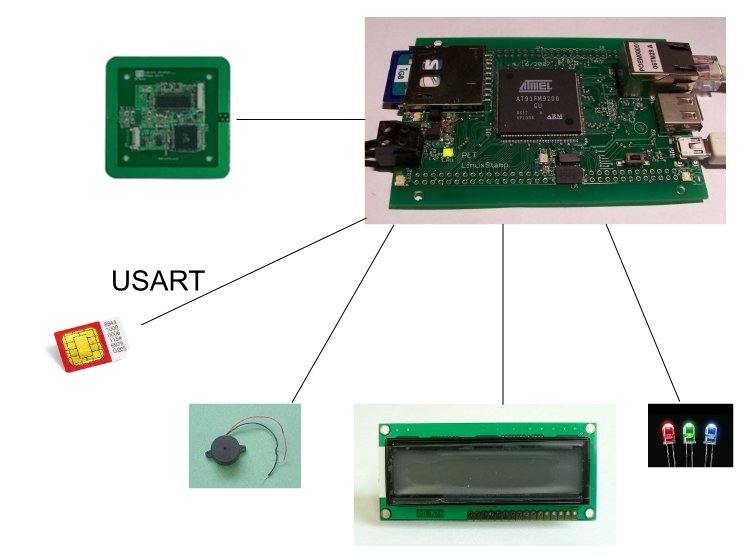
\includegraphics[scale=.25]{Imagenes/3.jpg} 
  \end{center}
  \caption{Solución considerada 4}\label{Fig:HW4} 
\end{figure}

Todos los periféricos se conectan a la SBC a través de sus interfaces nativas, esto incluye también el integrado CL RC632 de Philips \cite{RC632} (ver hoja de datos en el apéndice \ref{HD}). Se debe diseñar la antena para propagar la señal RF hacia las tarjetas.

\bigskip
\item[5 -] microcontrolador + lector de tarjetas RFID + lector de tarjetas de contacto + display + buzzer + leds
\bigskip

\begin{figure}[H]
\centering
  \begin{center}
  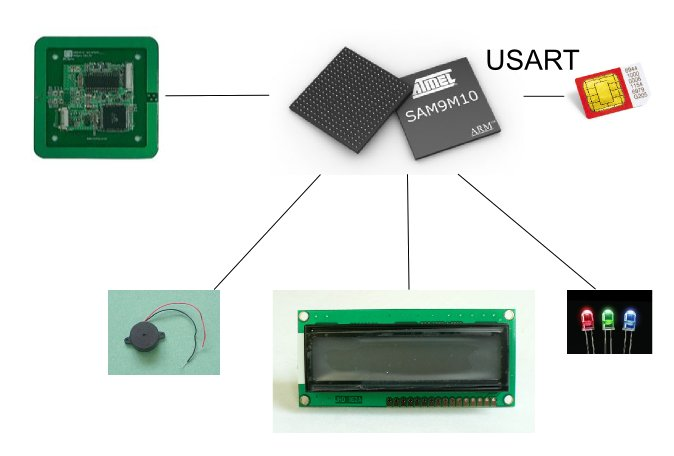
\includegraphics[scale=.25]{Imagenes/4.jpg} 
  \end{center}
  \caption{Solución considerada 5}\label{Fig:HW5} 
\end{figure}

Consta de un único PCB, que posee un microcontrolador como sistema central al cual se
conectan el resto de los dispositivos. Dicho PCB tiene incorporada la antena para la
propagación de RF.

\end{itemize}

\section{Arquitectura seleccionada}
En una primera instancia se pretendía utilizar únicamente el dispositivo OpenPCD (ver figura \ref{Fig:HW1}), ya que el mismo cuenta con un microcontrolador de la familia ARM, el AT91SAM7S128. Una vez estudiado se llegó a la conclusión de que no permitía la instalación de un sistema operativo GNU/Linux, ya que el mismo precisa más de 4 MB de RAM para poder hacer algo útil. Otra desventaja encontrada fue que sólo tiene un puerto I2C como forma de conectar periféricos.

Surgió entonces la necesidad de usar una SBC como dispositivo capaz de ejecutar un sistema operativo y las aplicaciones necesarias para que el dispositivo cumpla con los requerimientos exigidos. El dispositivo OpenPCD pasaría entonces a cumplir la función de lector/escritor de tarjetas RFID (ver figuras \ref{Fig:HW2} y \ref{Fig:HW3}), conectado a la SBC a través de su puerto USB, mientras que para el resto de los periféricos se diseñaría un PCB que fuera capaz de ser conectado a la SBC a través de sus interfaces nativas. Esta arquitectura fue descartada por el incremento en el costo del proyecto.

Fue necesario entonces descartar el uso del dispositivo OpenPCD y dar lugar a un diseño propio del lector/escritor de tarjetas RFID (ver figura \ref{Fig:HW4}), utilizando para esto el integrado CL RC632 de Philips.

La última opción y la más ambiciosa, plantea el diseño completo de un PCB (ver figura \ref{Fig:HW5}) conteniendo un microcontrolador y memoria capaz de ejecutar un sistema operativo, los lectores de tarjetas, tanto de contacto como RFID, y el resto de los periféricos (display, leds, buzzer). Esta opción fue dejada de lado por entender que excedería los plazos de tiempo del proyecto.

Se pensó entonces en diseñar la arquitectura 4 indicada en la figura \ref{Fig:HW4}, SBC + lector de tarjetas RFID + lector de tarjeta de contacto + display + buzzer + leds, y dado que se cuenta con un OpenPCD, la opción 3 mostrada en la figura \ref{Fig:HW3}, SBC + OpenPCD + lector de tarjetas de contacto + display + buzzer + leds, se dejaría como arquitectura alternativa si no se alcanzaran buenos resultados con el lector/escritor de tarjetas RFID.

\bigskip
Luego de estudiar ventajas y desventajas de las arquitecturas planteadas, se eligió la indicada en el ítem 4 en la sección \ref{arqEst}, que es la que más se adaptó a los requerimientos necesarios:

\begin{itemize}
\item SBC +  lector de tarjetas RFID + lector de tarjeta de contacto + display + buzzer + leds
\end{itemize}

En la figura \ref{Fig:HW_GRAL} se muestra un diagrama de bloques correspondiente a la arquitectura seleccionada:

\begin{figure}[H]
\centering
  \begin{center}
  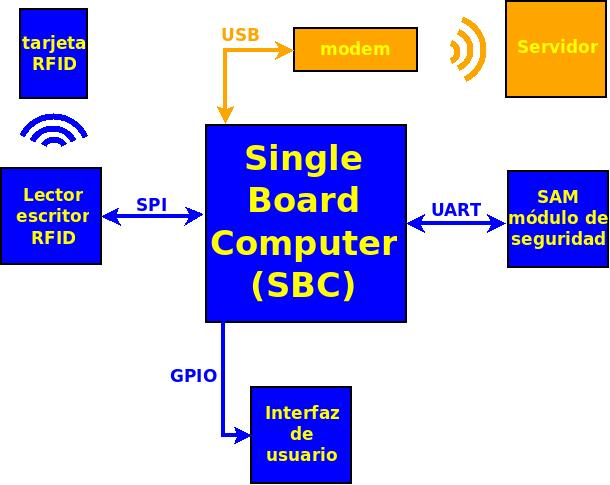
\includegraphics[scale=.5]{Imagenes/diagrama_rf2.jpg} 
  \end{center}
  \caption{Diagrama de bloques de la arquitectura seleccionada}\label{Fig:HW_GRAL} 
\end{figure}


Los bloques oscuros serán implementados, no así los claros.

\bigskip
Como se mencionó en el punto \ref{2.2}, el bloque de la figura \ref{Fig:HW_GRAL} referente al módulo de seguridad, no está operativo en la aplicación final. 
La comunicación con un servidor no está implementada por quedar fuera del alcance del proyecto.

\newpage
\section{Elecci\'on de hardware}

\subsection{SBC}
En primera instancia se confeccionó una lista con posibles candidatas de SBC disponibles
en el mercado internacional, teniendo en cuenta factores como: precio, puertos de I/O, memoria RAM, memoria Flash, puertos USB, soporte para GNU/Linux, entre otros.
Se definieron una serie de requisitos mínimos necesarios para seleccionar de la lista la SBC que más se adecuara a la arquitectura definida.
Para la comunicación con el resto de los módulos será necesario: una interfaz UART para el módulo de seguridad (SAM); una interfaz SPI para el módulo lector/escritor RFID (CL RC632 de Philips); 20 GPIO para display, leds, buzzer, otros; 1 USB host para una posible conexión de un modem 3G (intercambio de datos con un servidor). En cuanto a la memoria disponible, tomando como referencia el AFE, debe ser de 32 MB de RAM y 8 MB de flash para un funcionamiento aceptable. Es conveniente, pensando a futuro, que el procesador trabaje a una frecuencia no menor a 200 MHz.
Dado el presupuesto estimado para el proyecto, el precio no debe superar los 150 dólares en origen.
Como requisito adicional se exigió que existiera un foro actualizado y soporte técnico que permitiera evacuar dudas.


Aplicados los requisitos mínimos a la lista previamente confeccionada de SBC candidatas, se optó por dos: GESBC-9G20 \cite{9G20} y Hawkboard \cite{Hawk}.
En cuanto a la primera opción, GESBC-9G20, los fabricantes no respondieron consultas, por tanto se descartó. Se optó entonces por la segunda opción, Hawkboard, puesto que respondieron a las consultas en tiempos razonables y se logró evacuar dudas desde el foro.


Luego de comprar dos Hawkboard, ambas resultaron defectuosas a nivel de hardware, después de varios meses de pruebas sin resultados y sin respuestas concretas por parte del proveedor y fabricante y con la intención de cumplir con los plazos del proyecto, se optó por utilizar una SBC (Beagleboard \cite{Beagle}) que se consiguió en préstamo por medio del INCO. Esta SBC cumplió con los requisitos mínimos, aunque en ese momento tenía un costo del doble de la Hawkboard, teniéndose que diseñar un módulo hardware adicional.
Finalmente, la SBC seleccionada para trabajar fue la Beagleboard rev.C4.

Las características generales de la BeagleBoard son: cuenta con un procesador \\
OMAP3530 de 720 MHz con arquitectura ARM. Posee  memoria NAND-flash de 256 MB y memoria ROM de igual tamaño. Tiene una ranura adicional para extender la memoria a través de una memoria SD. Entre otras cosas cuenta con un puerto USB OTG, un puerto USB host, un bloque de expansión de 28 pines (con señales a 1,8 Volt), puerto JTAG, conector RS232, etc.\\
En lo que respecta a la potencia disipada, la Beagleboard tiene un consumo de pico de 2W, y un consumo promedio de 560mW \cite{consumo1} \cite{consumo2}.

\begin{figure}[H]
  \centering
  \subfigure[Vista anversa de la SBC]{\label{sbcF}
  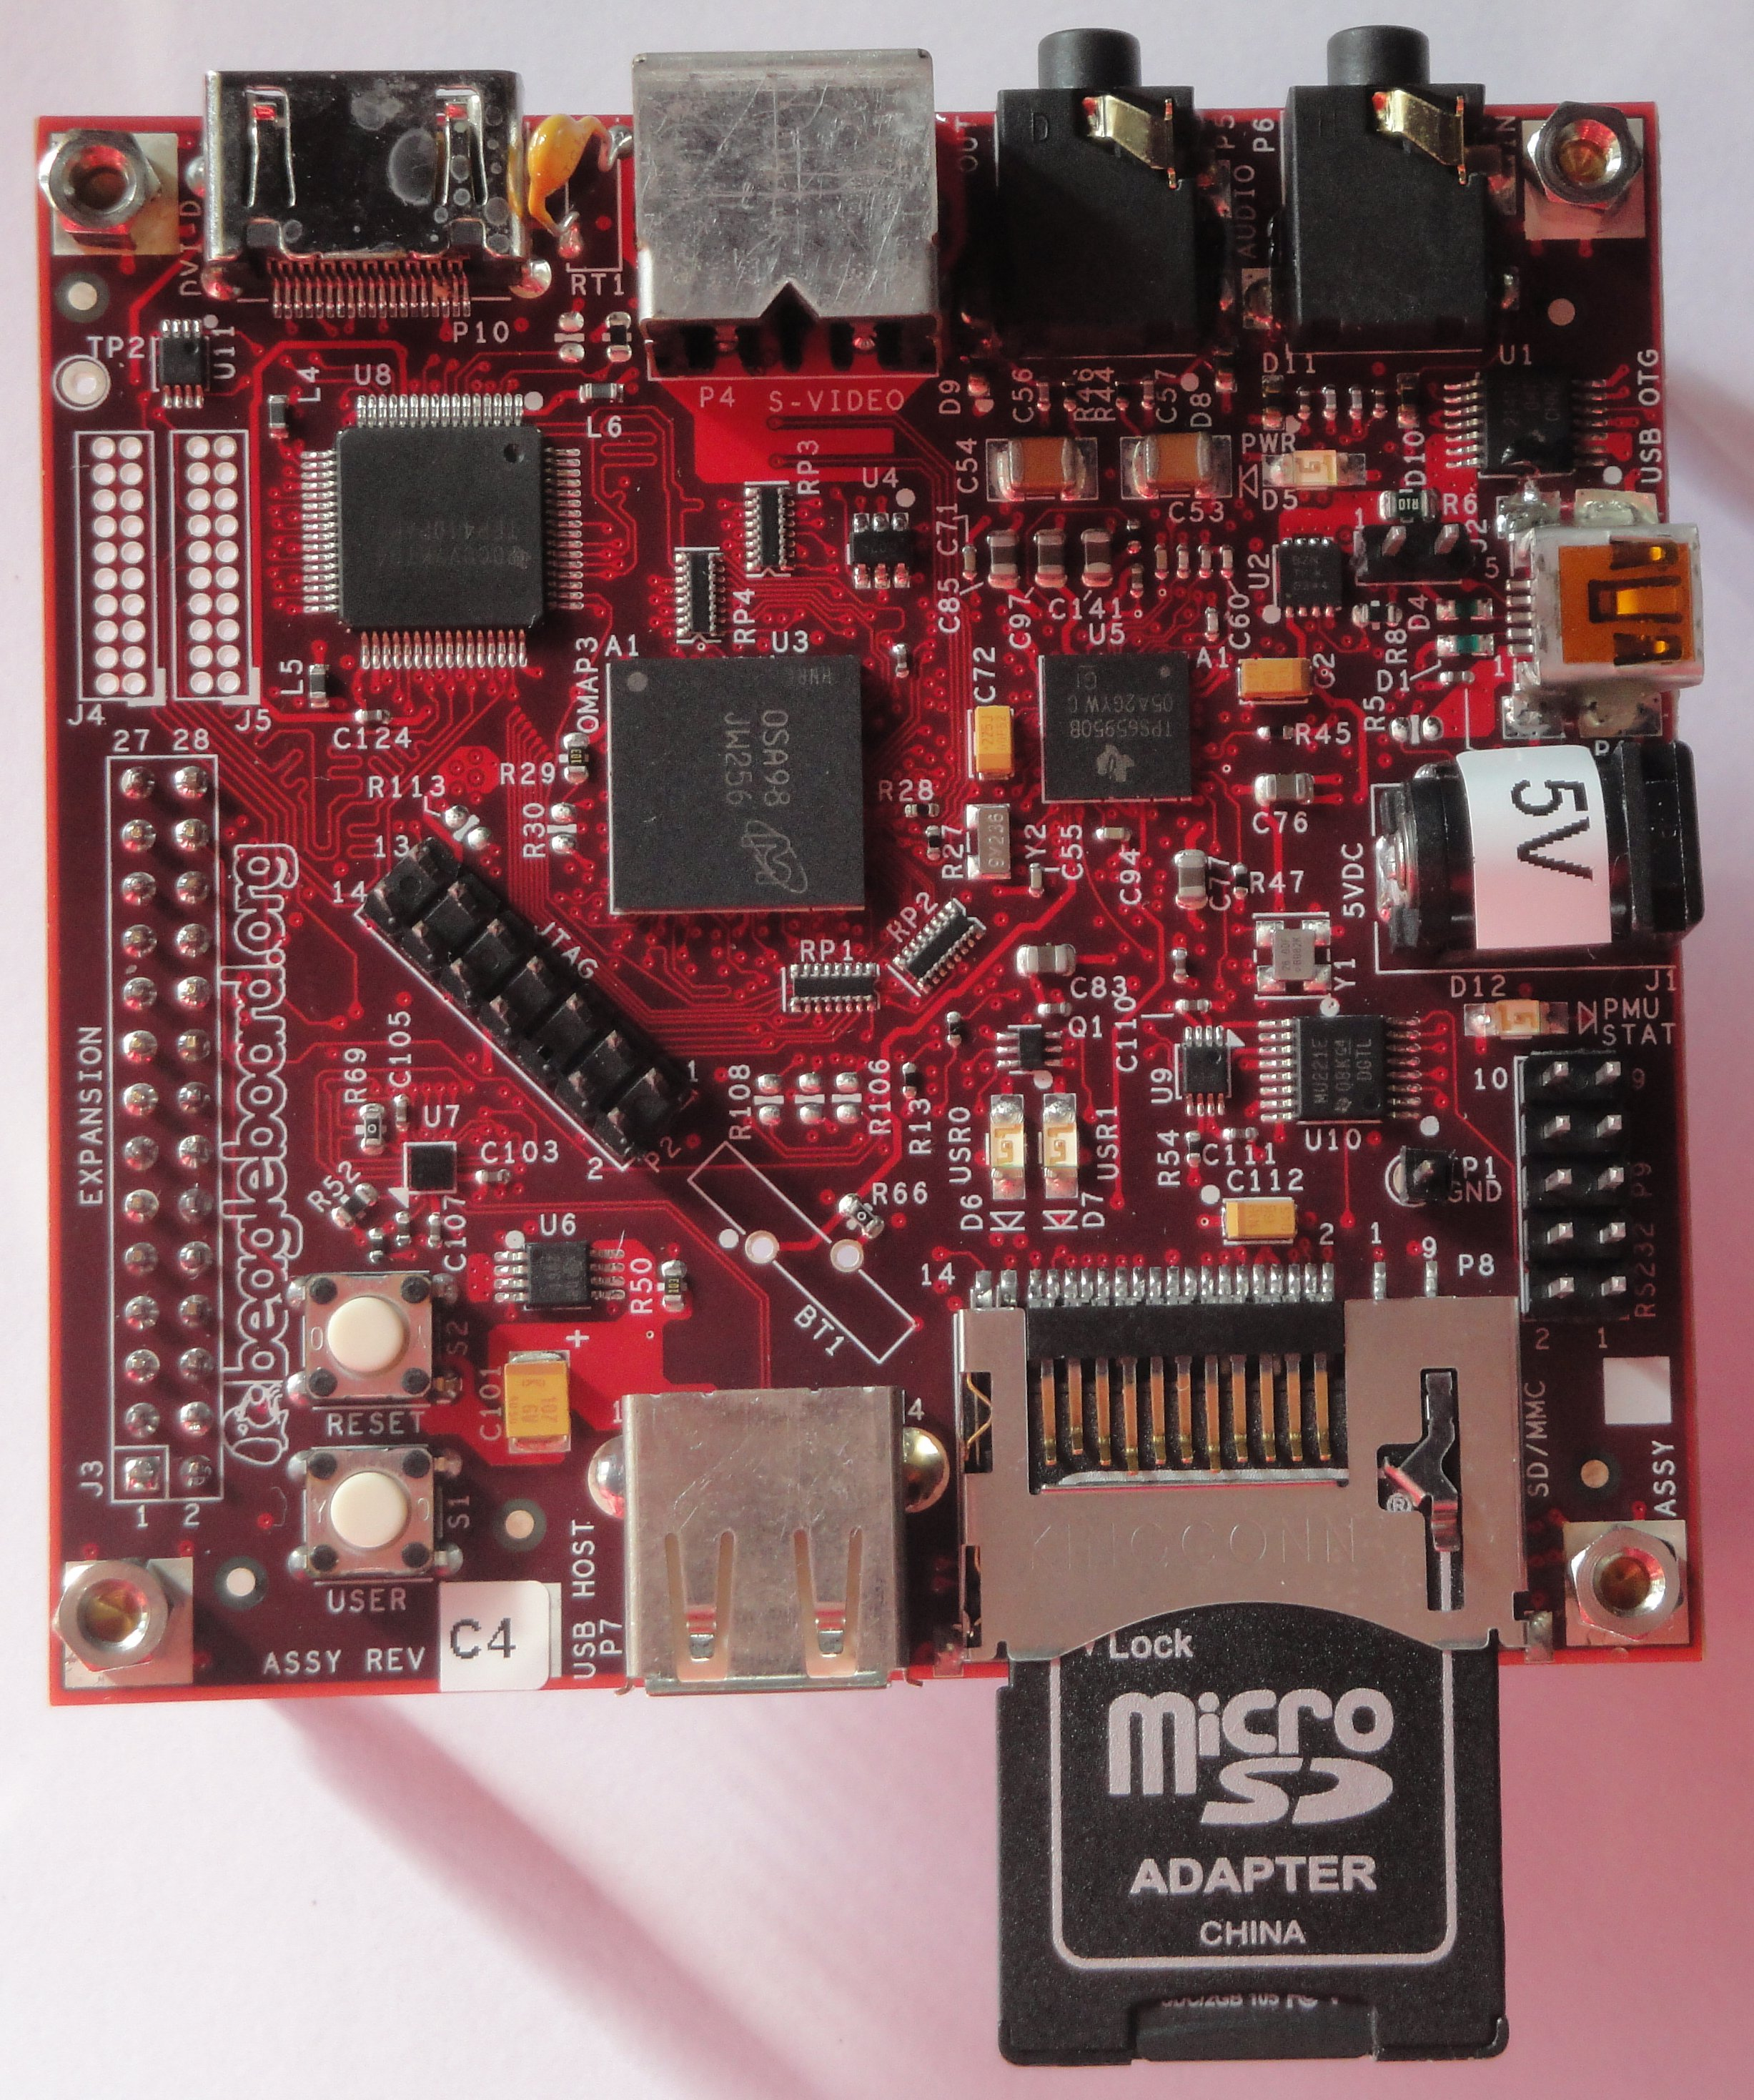
\includegraphics[scale=.08]{Imagenes/SBC_f.jpg} } 
  \subfigure[Vista reversa de la SBC]{\label{sbcB} 
  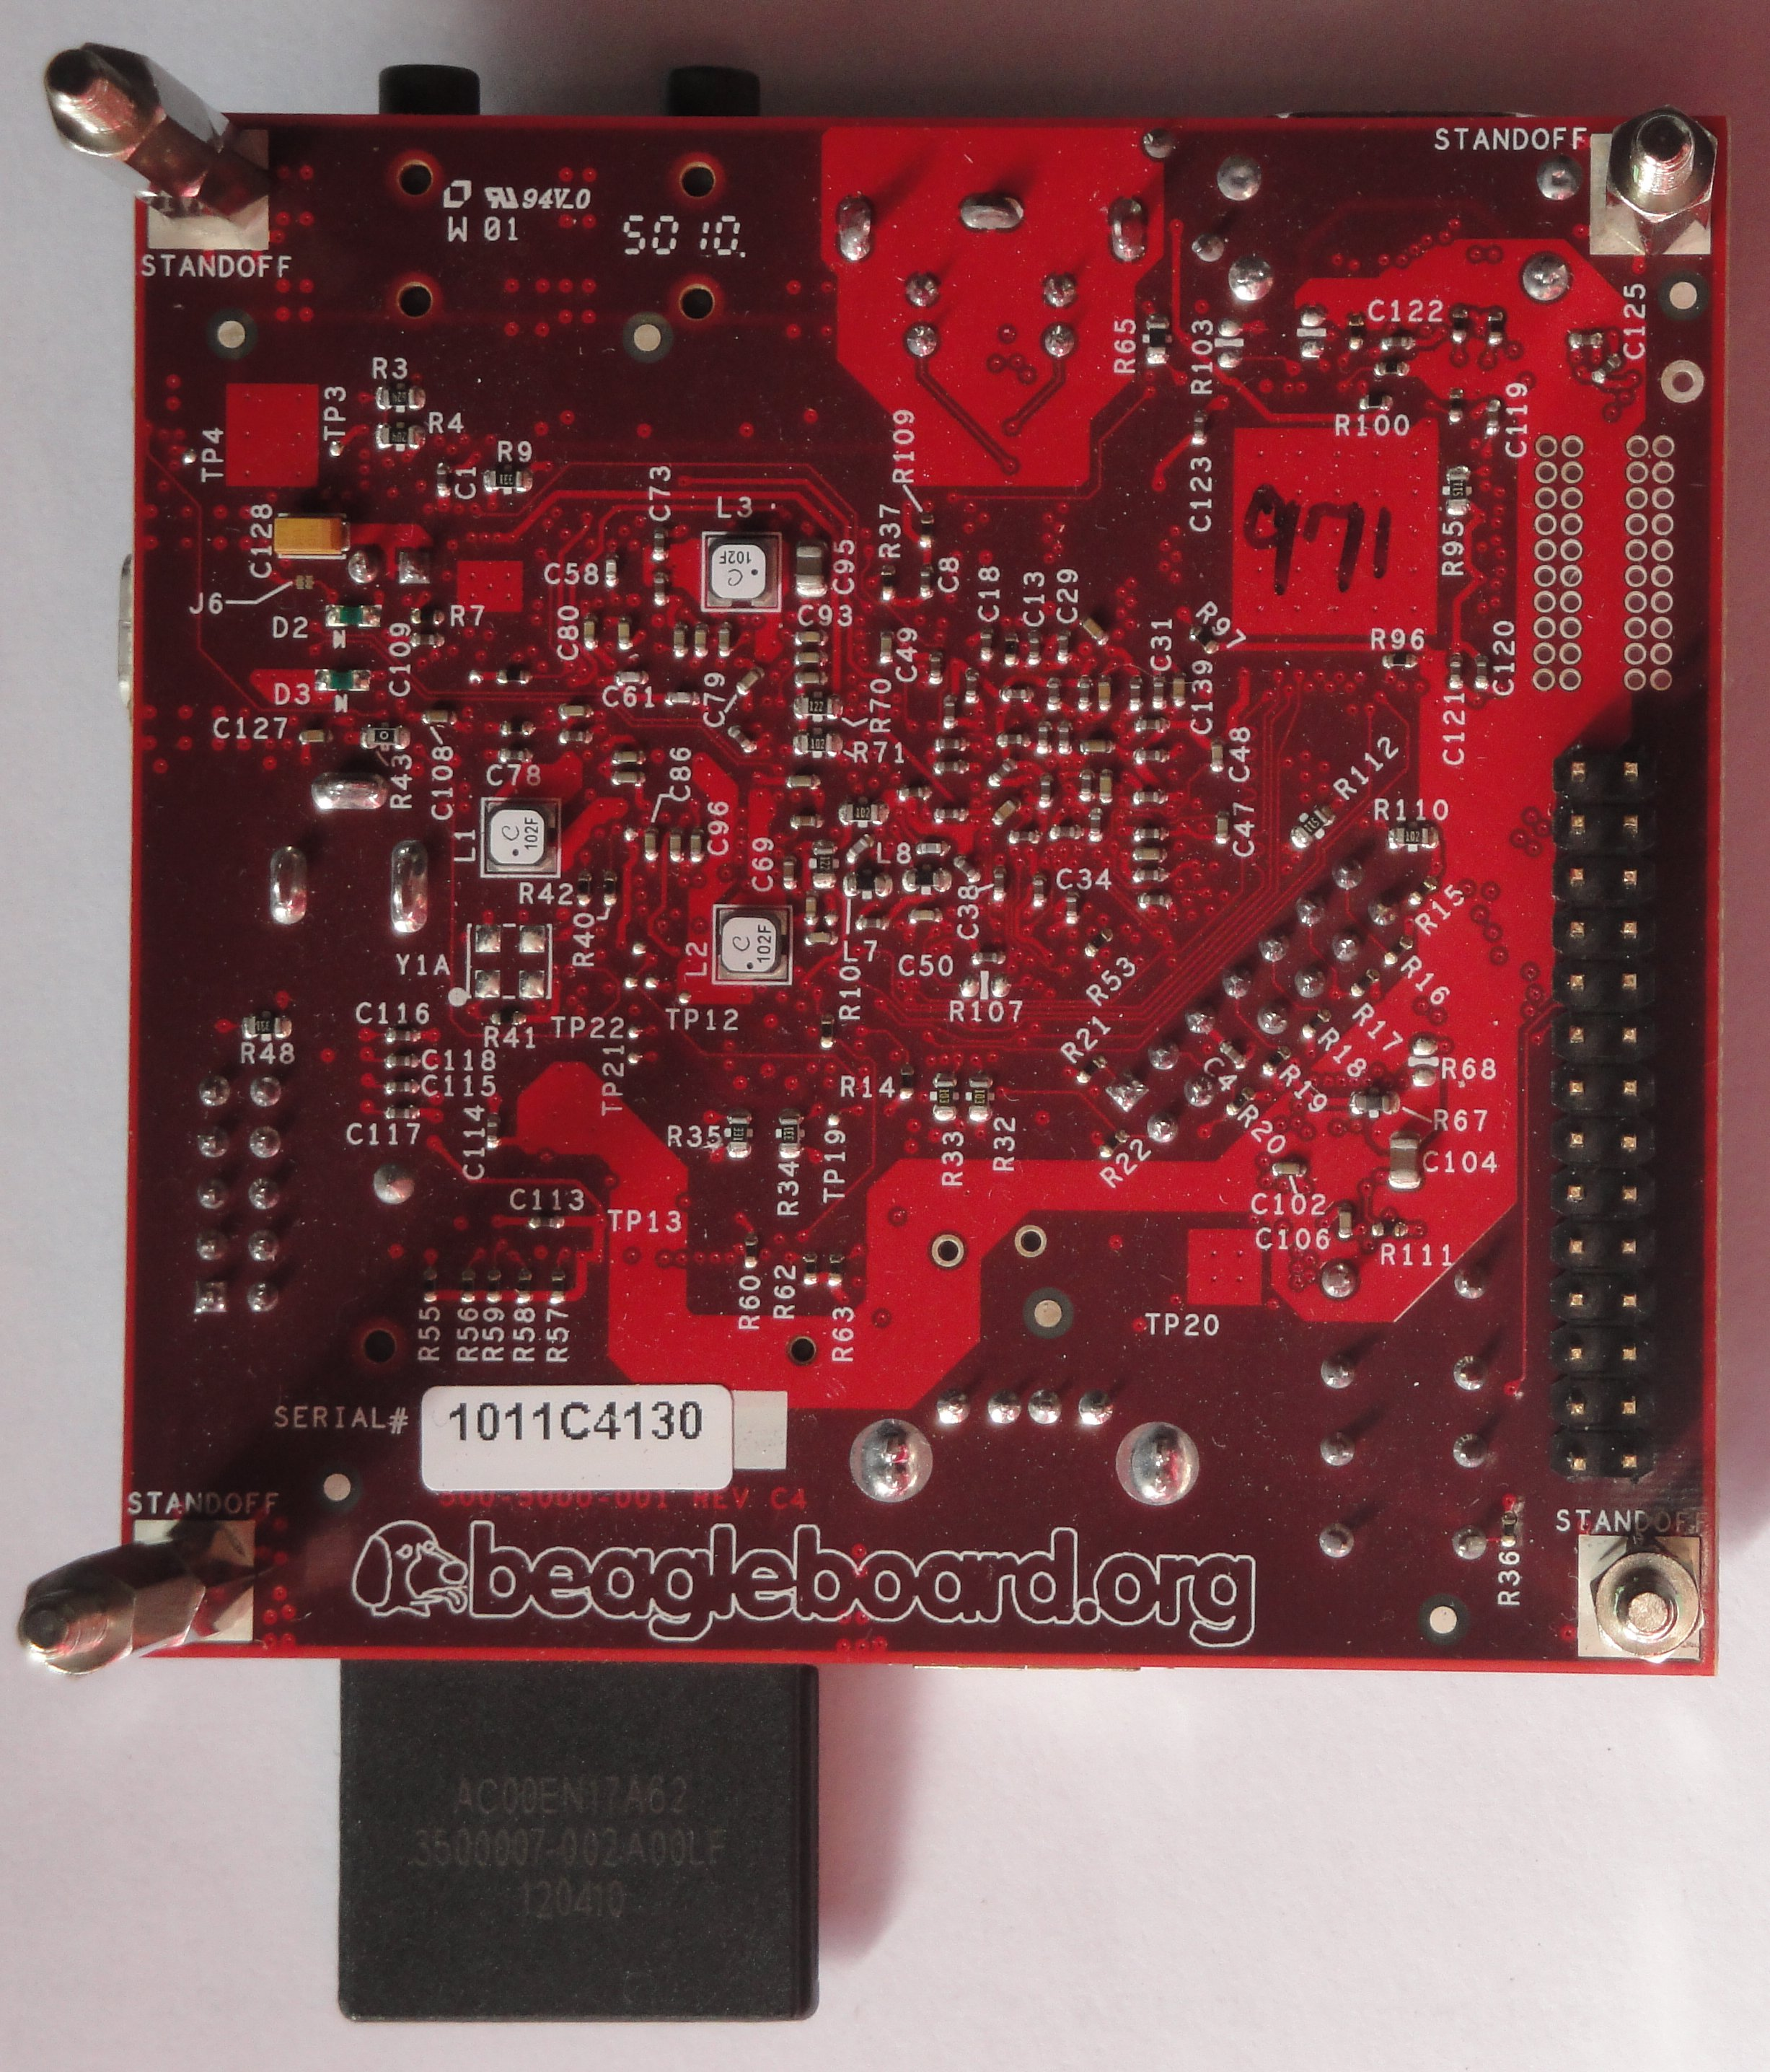
\includegraphics[scale=.08]{Imagenes/SBC_b.jpg} }

  \caption{Vista anversa y reversa de la SBC}\label{sbcFB}
\end{figure}


\subsection{VLT - Conversor de Voltajes}
Este módulo no fue tenido en cuenta en la primera etapa del diseño de la arquitectura hardware, sino que surge como necesidad debido al cambio de SBC. Como consecuencia de lo anterior se vio la ventaja de incorporar una placa que permite la conexión entre la SBC y el resto del hardware, el cual puede permanecer inalterado por más que no ocurra lo mismo con la SBC, ya que ésta puede cambiar de versión o dejar de fabricarse en un breve lapso de tiempo. El único elemento a cambiar sería entonces la placa VLT, que es más simple y barata de fabricar que las restantes partes.
La placa de circuito impreso VLT consta básicamente de dos conectores, uno de ellos permite la conexión con la Beagleboard y el otro la conexión con el restante hardware el cual se encuentra intergrado en un PCB llamdo SCUI. Ambos conectores no se encuentran directamente interconectados entre sí a través de pistas, pues para el caso particular de Beagleboard fue necesario incorporar conversores de tensión que permitieran el traslado del nivel de tensión desde 1,8 Volt que usa esta SBC, a las tensiones con las que operan los periféricos, ya sea 3,3 o 5 Volt.
El último elemento, no menos importante, es un regulador de tensión LDO que permite generar 3,3 Volt a partir de la fuente de tensión de 5 Volt de la propia Beagleboard.

Por más detalles ver esquemático en la figura \ref{Fig:VLT}.

\begin{figure}[H]
  \centering
  \subfigure[Vista anversa de la SBC]{\label{vltF}
  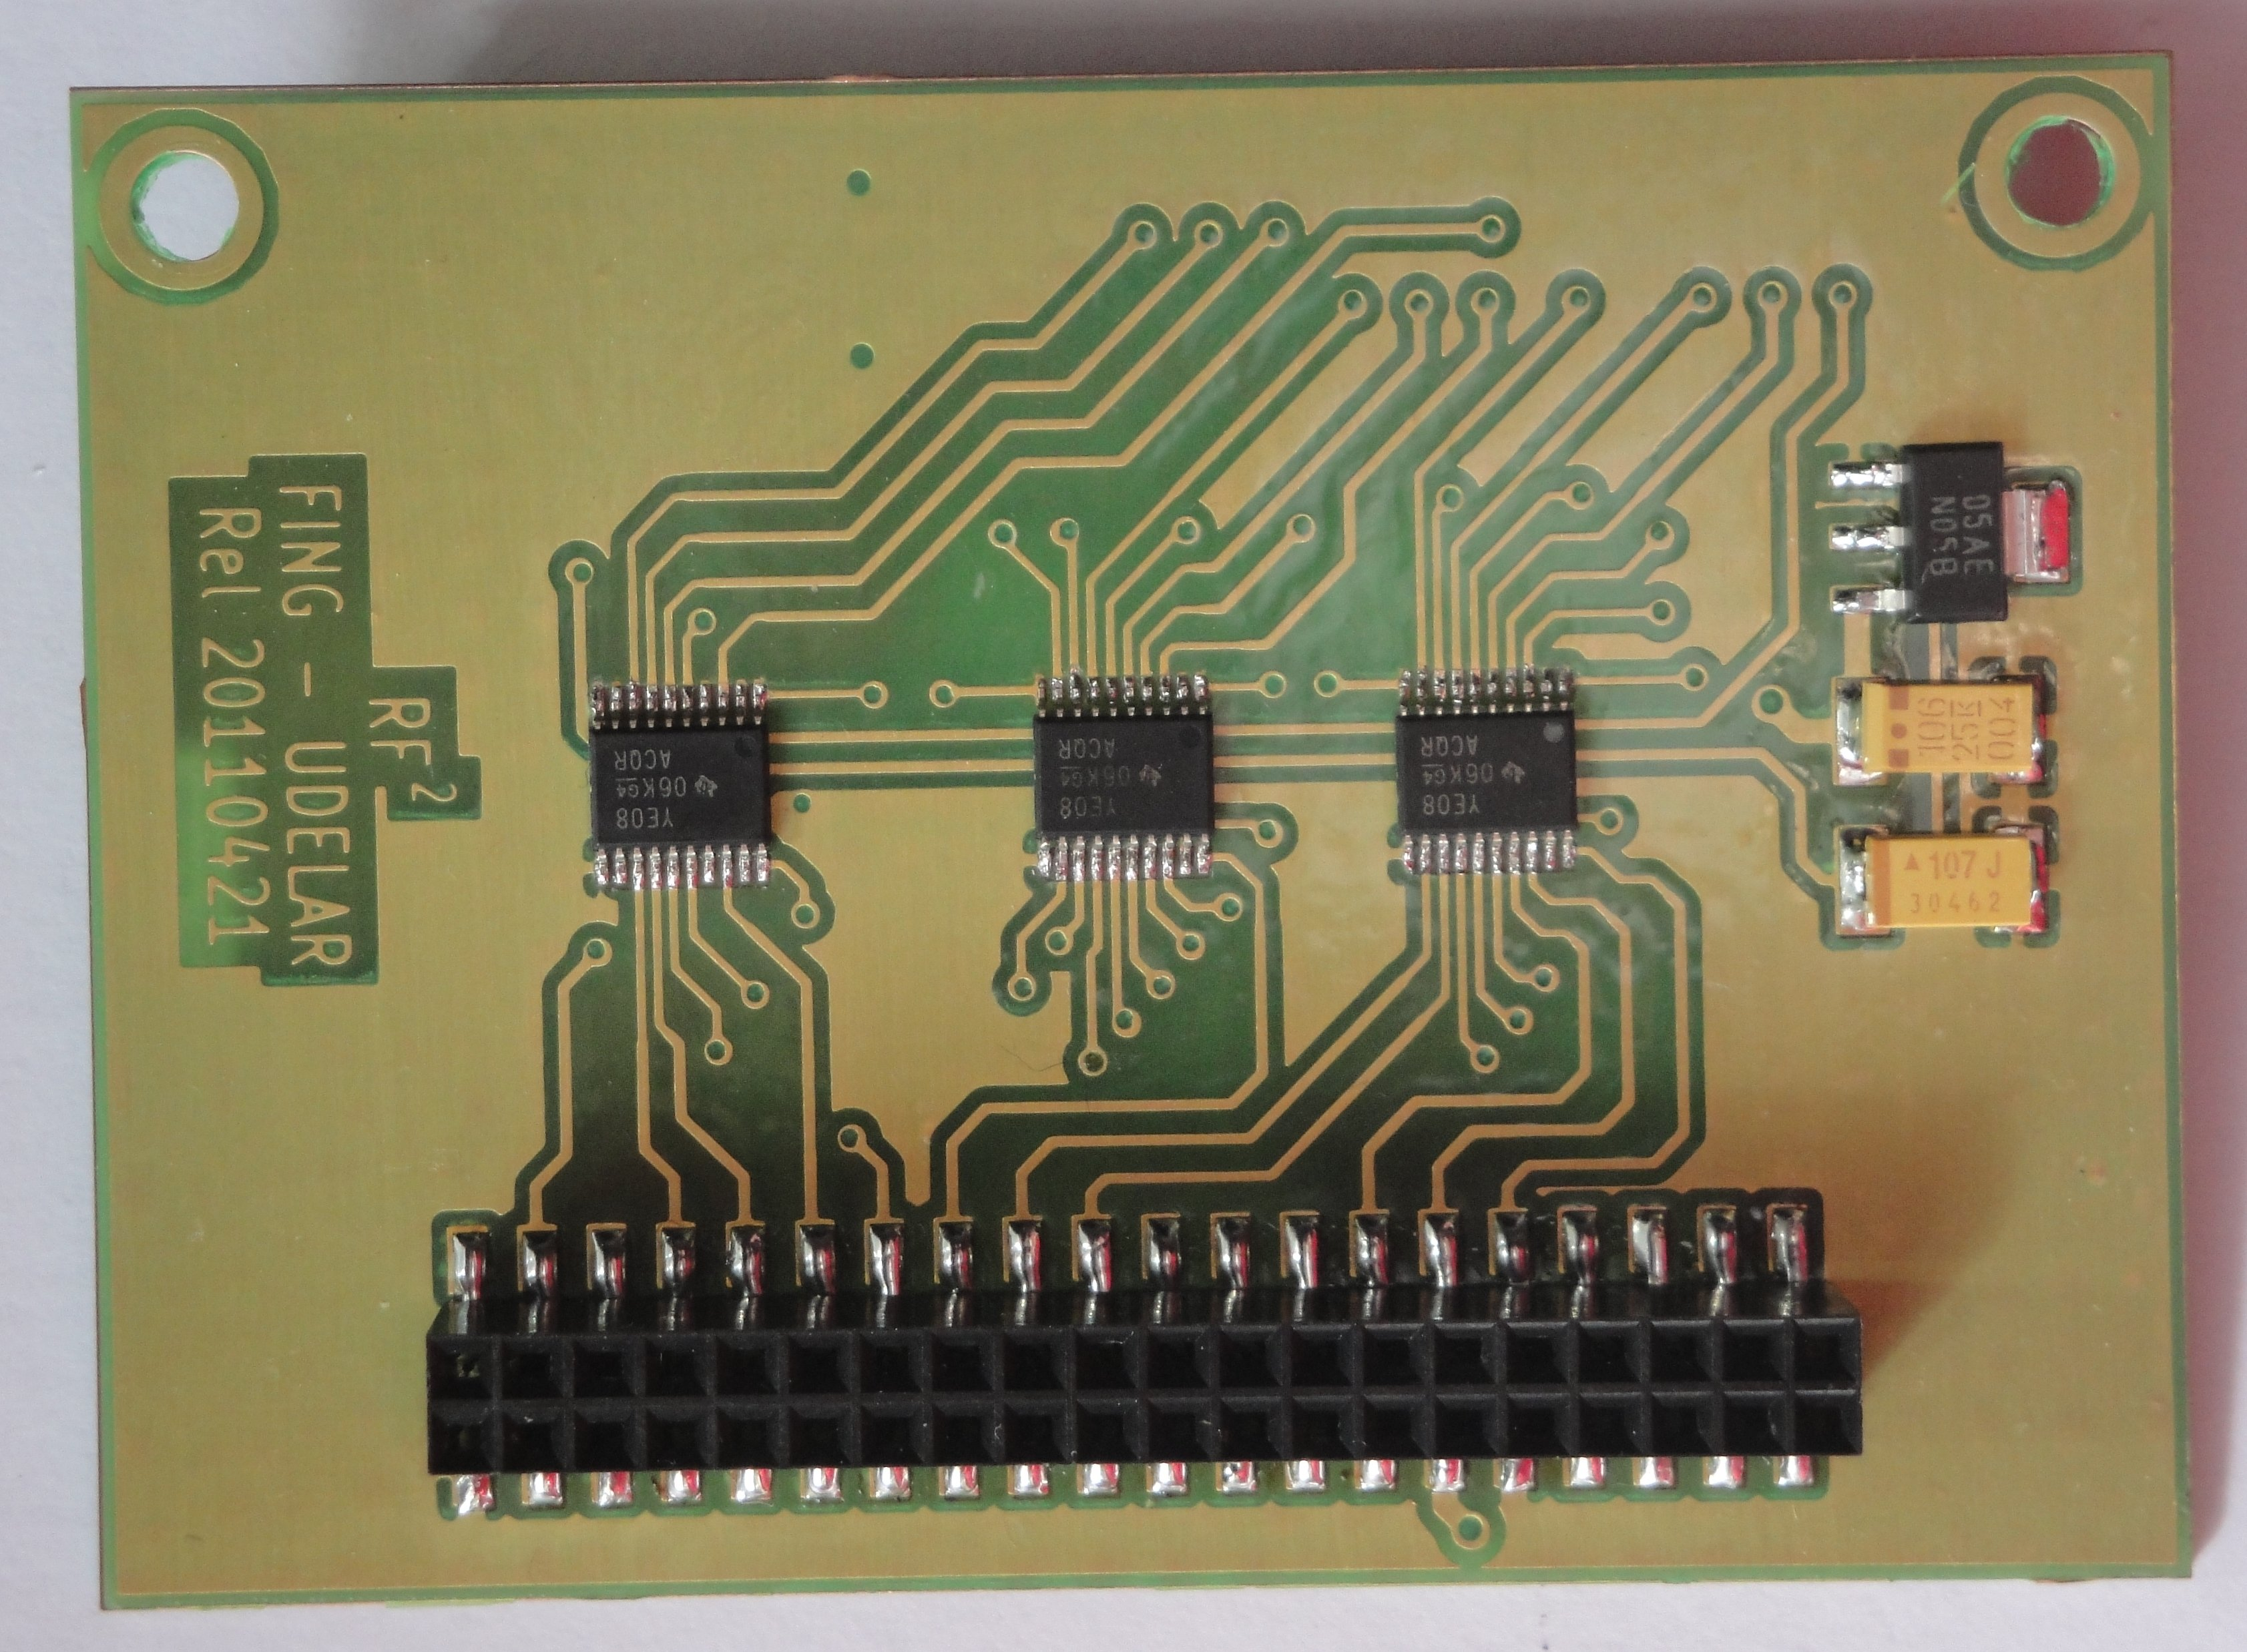
\includegraphics[scale=.08, angle=90]{Imagenes/VLT_f.jpg} } 
  \subfigure[Vista reversa de la SBC]{\label{vltB} 
  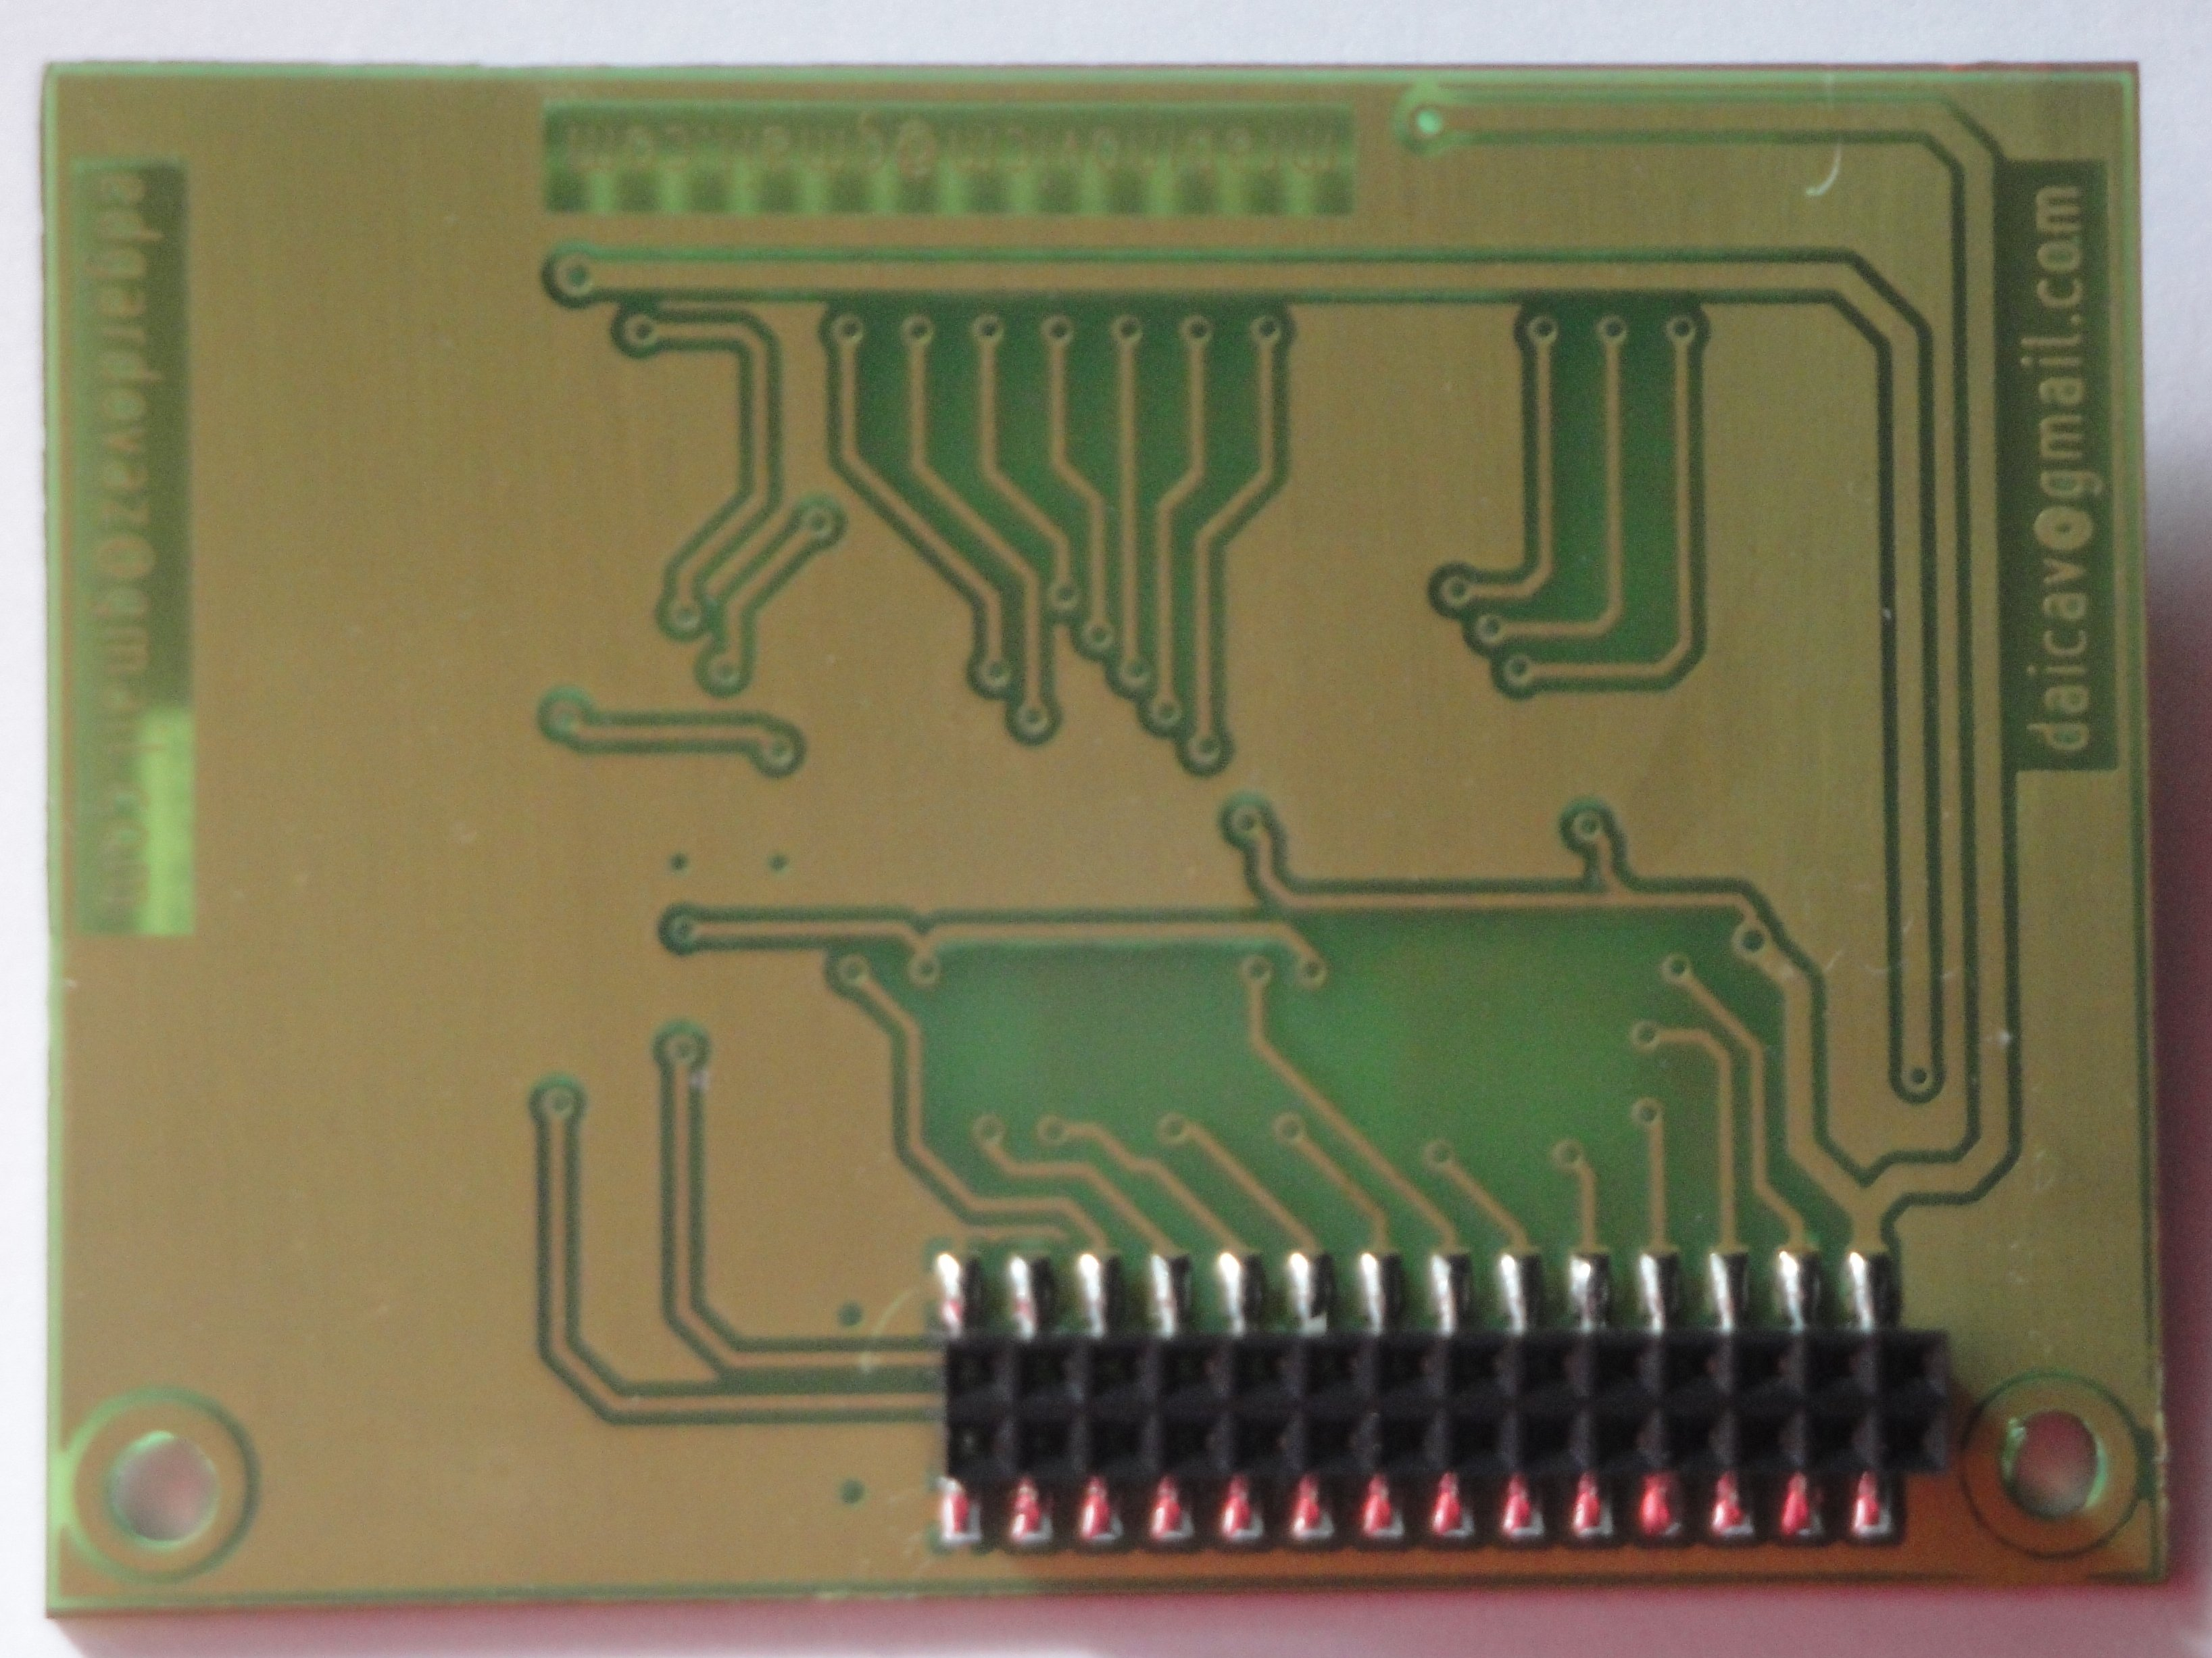
\includegraphics[scale=.08, angle=90]{Imagenes/VLT_b.jpg} }

  \caption{Vista anversa y reversa de VLT}\label{vltFB}
\end{figure}

\subsection{SCUI - Lector de tarjetas de contacto e Interfaz de Usuario}
El módulo SCUI puede dividirse en dos partes, una de ellas es un lector de tarjetas de contacto basadas en la norma ISO7816, y la otra es una simple interfaz para el usuario.
El lector de tarjetas de contacto (smart cards), está compuesto por un conversor full duplex a half duplex el cual se encuentra conectado a uno de los puertos UART de la SBC a través del módulo VLT, que se describió en el punto anterior. Este conversor permite la transmisión de datos directamente entre la tarjeta y la SBC, sin necesidad de intercalar un ASIC para el manejo de tarjetas del tipo ISO7816. Cuenta también con un oscilador para alimentar la entrada de reloj de las tarjetas. La entrada de control (OE) del oscilador operada desde la SBC permite poner la salida de reloj en tercer estado, cosa muy útil a la hora de cumplir con la secuencia de inicialización de las tarjetas descritas en el estándar. El lector permite operar con tarjetas clase A (alimentadas a 5 Volt) y clase B (alimentadas a 3,3 Volt) haciendo uso de un jumper que permite intercambiar la tensión de alimentación suministrada a la tarjeta. Se cuenta con un zócalo para insertar la tarjeta de contacto.
Por más detalles ver esquemático en la figura \ref{Fig:SAM}.

Por otra parte, la intefaz de usuario está compuesta por tres leds (verde, amarillo y rojo), buzzer y un display LCD16x2 donde son desplegados los mensajes que indican al usuario la operación que se efectúa sobre su tarjeta Mifare.
Por más detalles ver esquemático en la figura \ref{Fig:UI}.

El último elemento a describir aquí es un conector receptáculo 5x2 (100mils) en el que se conecta el módulo lector/escritor RFID que opera con las tarjetas RFID Mifare.
Por más detalles ver esquemático en la figura \ref{Fig:SCUI}.

\begin{figure}[H]
  \centering
  \subfigure[Vista anversa de SCUI]{\label{scuiF}
  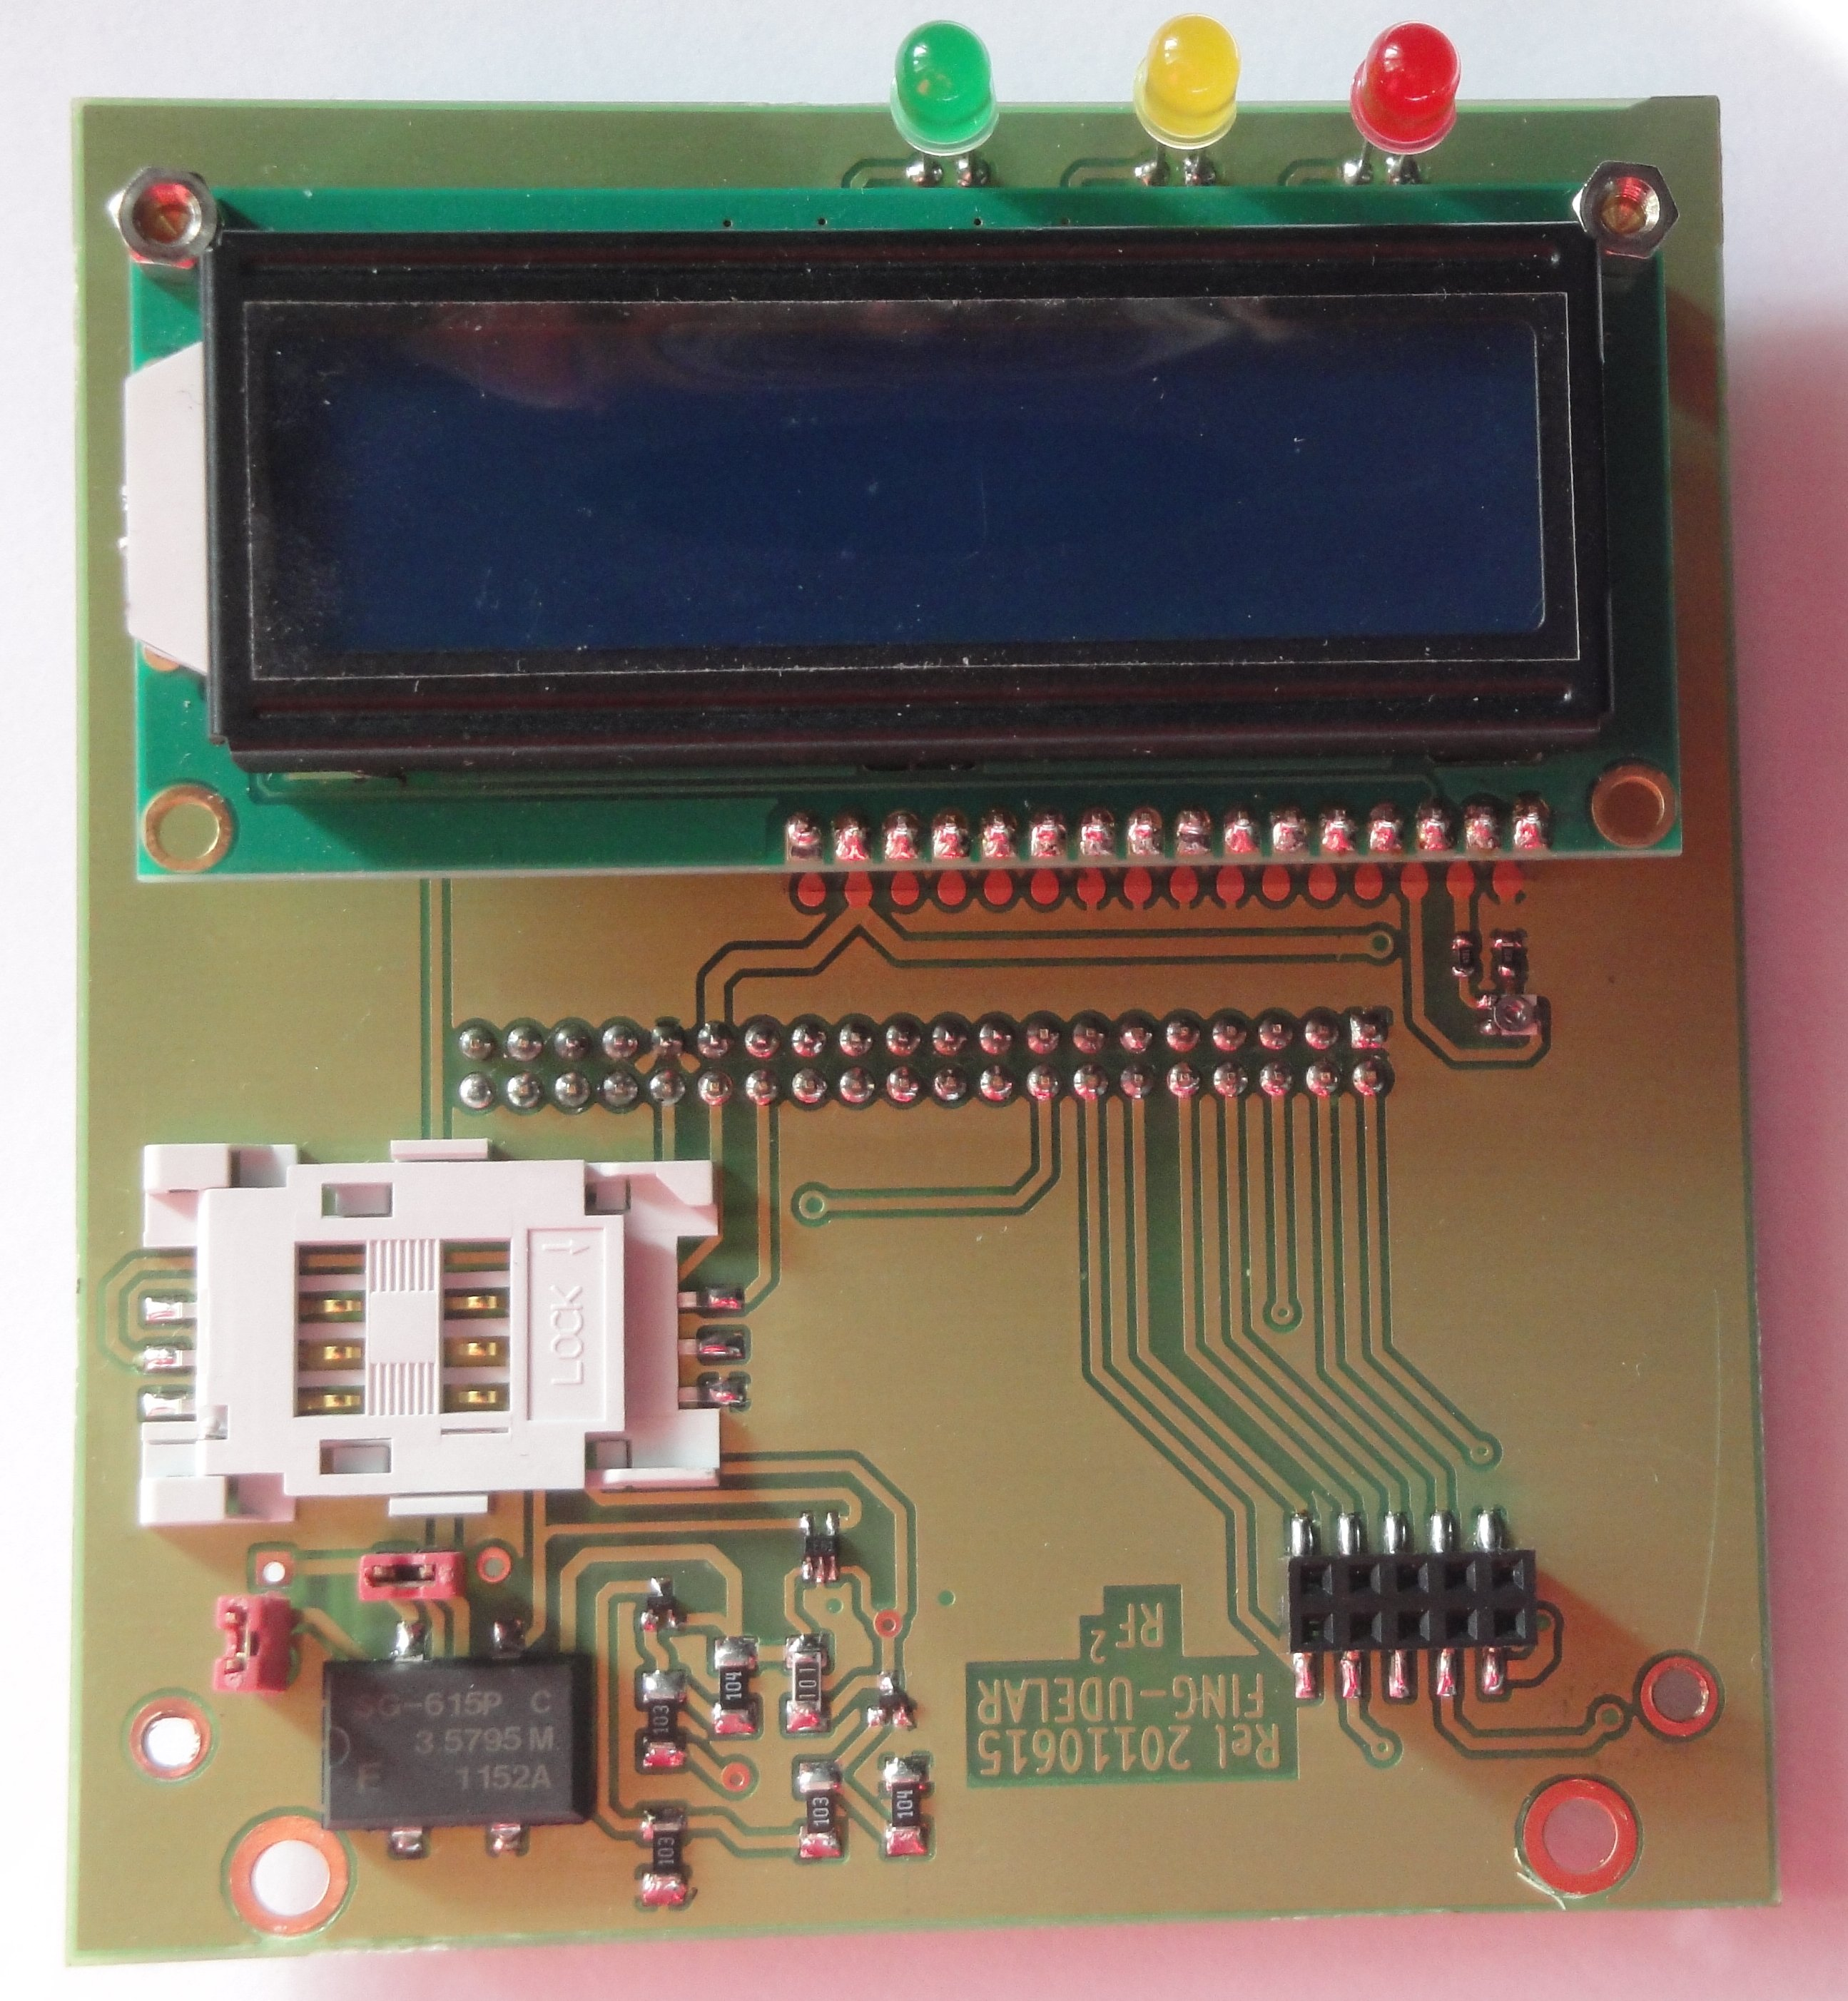
\includegraphics[scale=.07]{Imagenes/SCUI_f.jpg} } 
  \subfigure[Vista reversa de SCUI]{\label{scuiB} 
  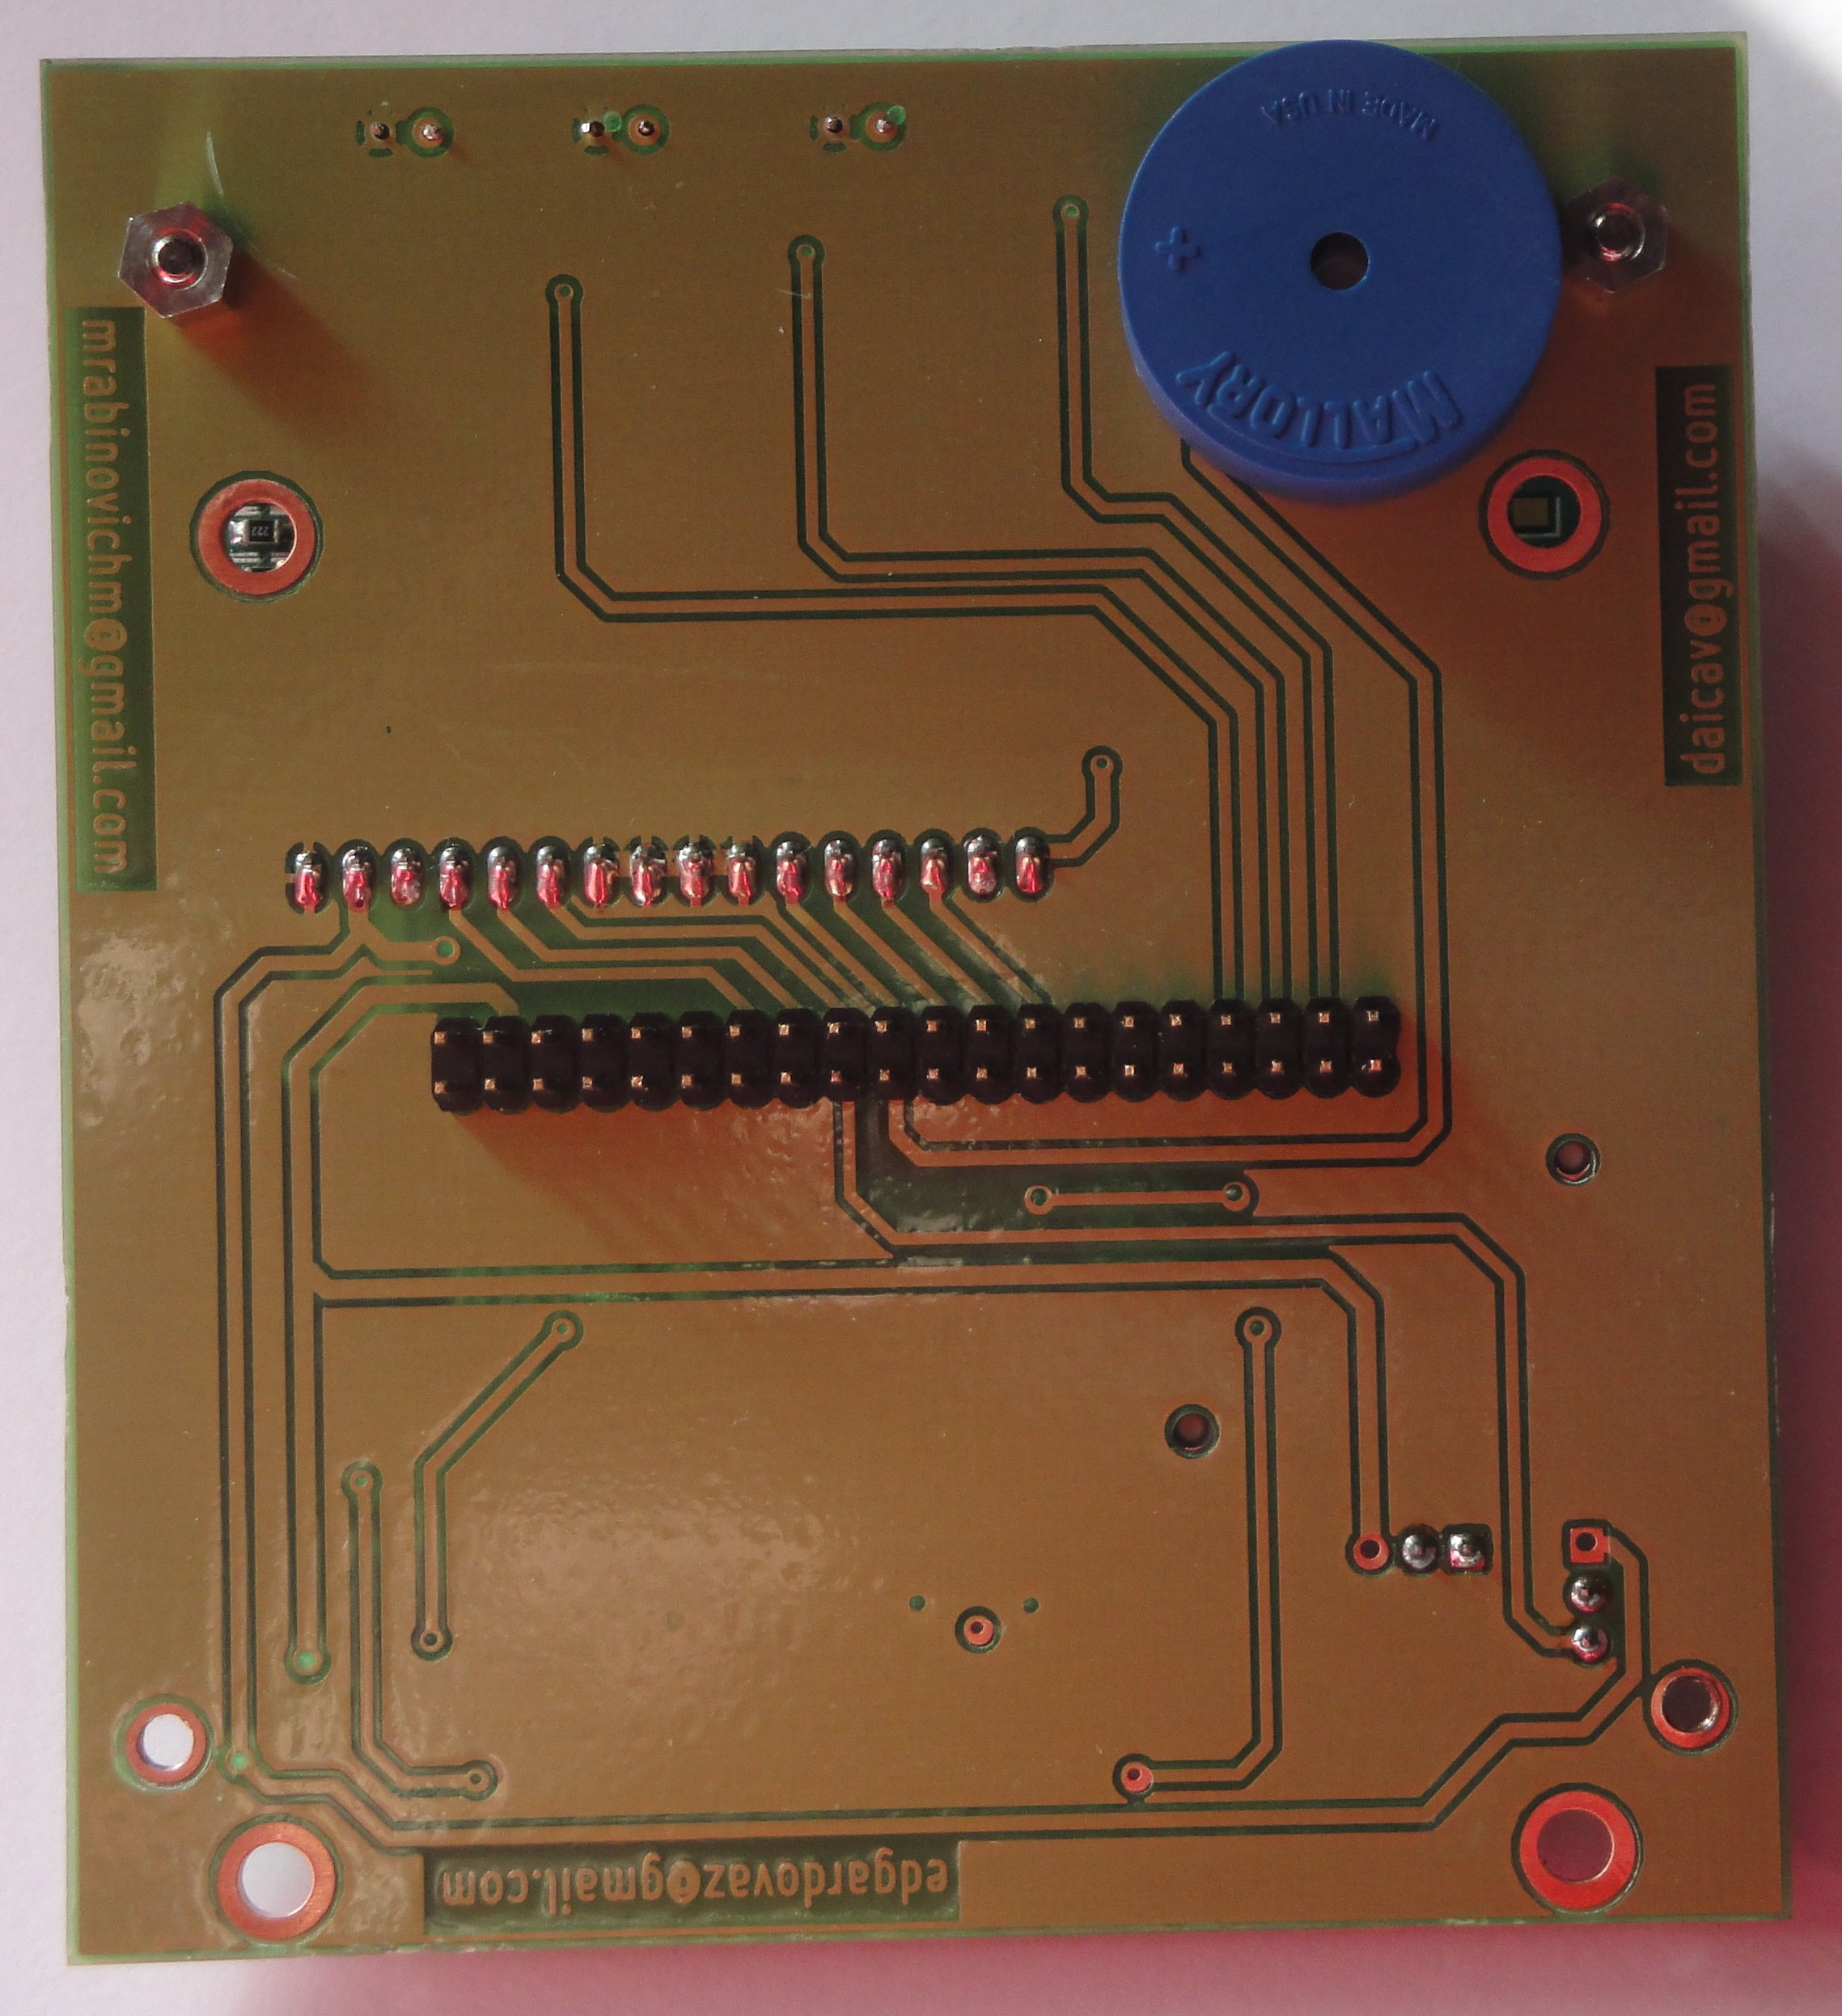
\includegraphics[scale=.08]{Imagenes/SCUI_b.jpg} }

  \caption{Vista anversa y reversa de SCUI}\label{scuiFB}
\end{figure}

\newpage
\subsection{Lector/Escritor RFID}
Este módulo es el encargado de la comunicación con las tarjetas RFID que cumplen con la norma ISO14443. Consta básicamente de cuatro secciones entre las que se encuentran: el integrado CL RC632; el filtro EMC, el circuito de adaptación de impedancia (matching); y el inductor de la antena. 
El ASIC CL RC632 permite, por un lado la comunicación digital con un microprocesador a través de su puerto de datos y por el otro lado la transmisión de datos hacia la antena que emitirá la señal RF para la comunicación con las tarjetas ISO14443.
Por más detalles ver esquemático en la figura \ref{Fig:RFID}.

Lo que se llama propiamente antena RF está conformada por el circuito de adaptación de impedancia (matching) y por el inductor, que propaga el campo magnético para lograr el acoplamiento necesario entre lector y tarjeta, de aquí la sigla PCD (Proximity Coupling Device).
Por más detalles ver esquemático en la figura \ref{Fig:RFID2}.

Los principios básicos de funcionamiento de la antena se detallan en el apéndice \ref{anx_antena}.

\begin{figure}[H]
  \centering
  \subfigure[Vista anversa del lector/escritor RFID]{\label{scuiF}
  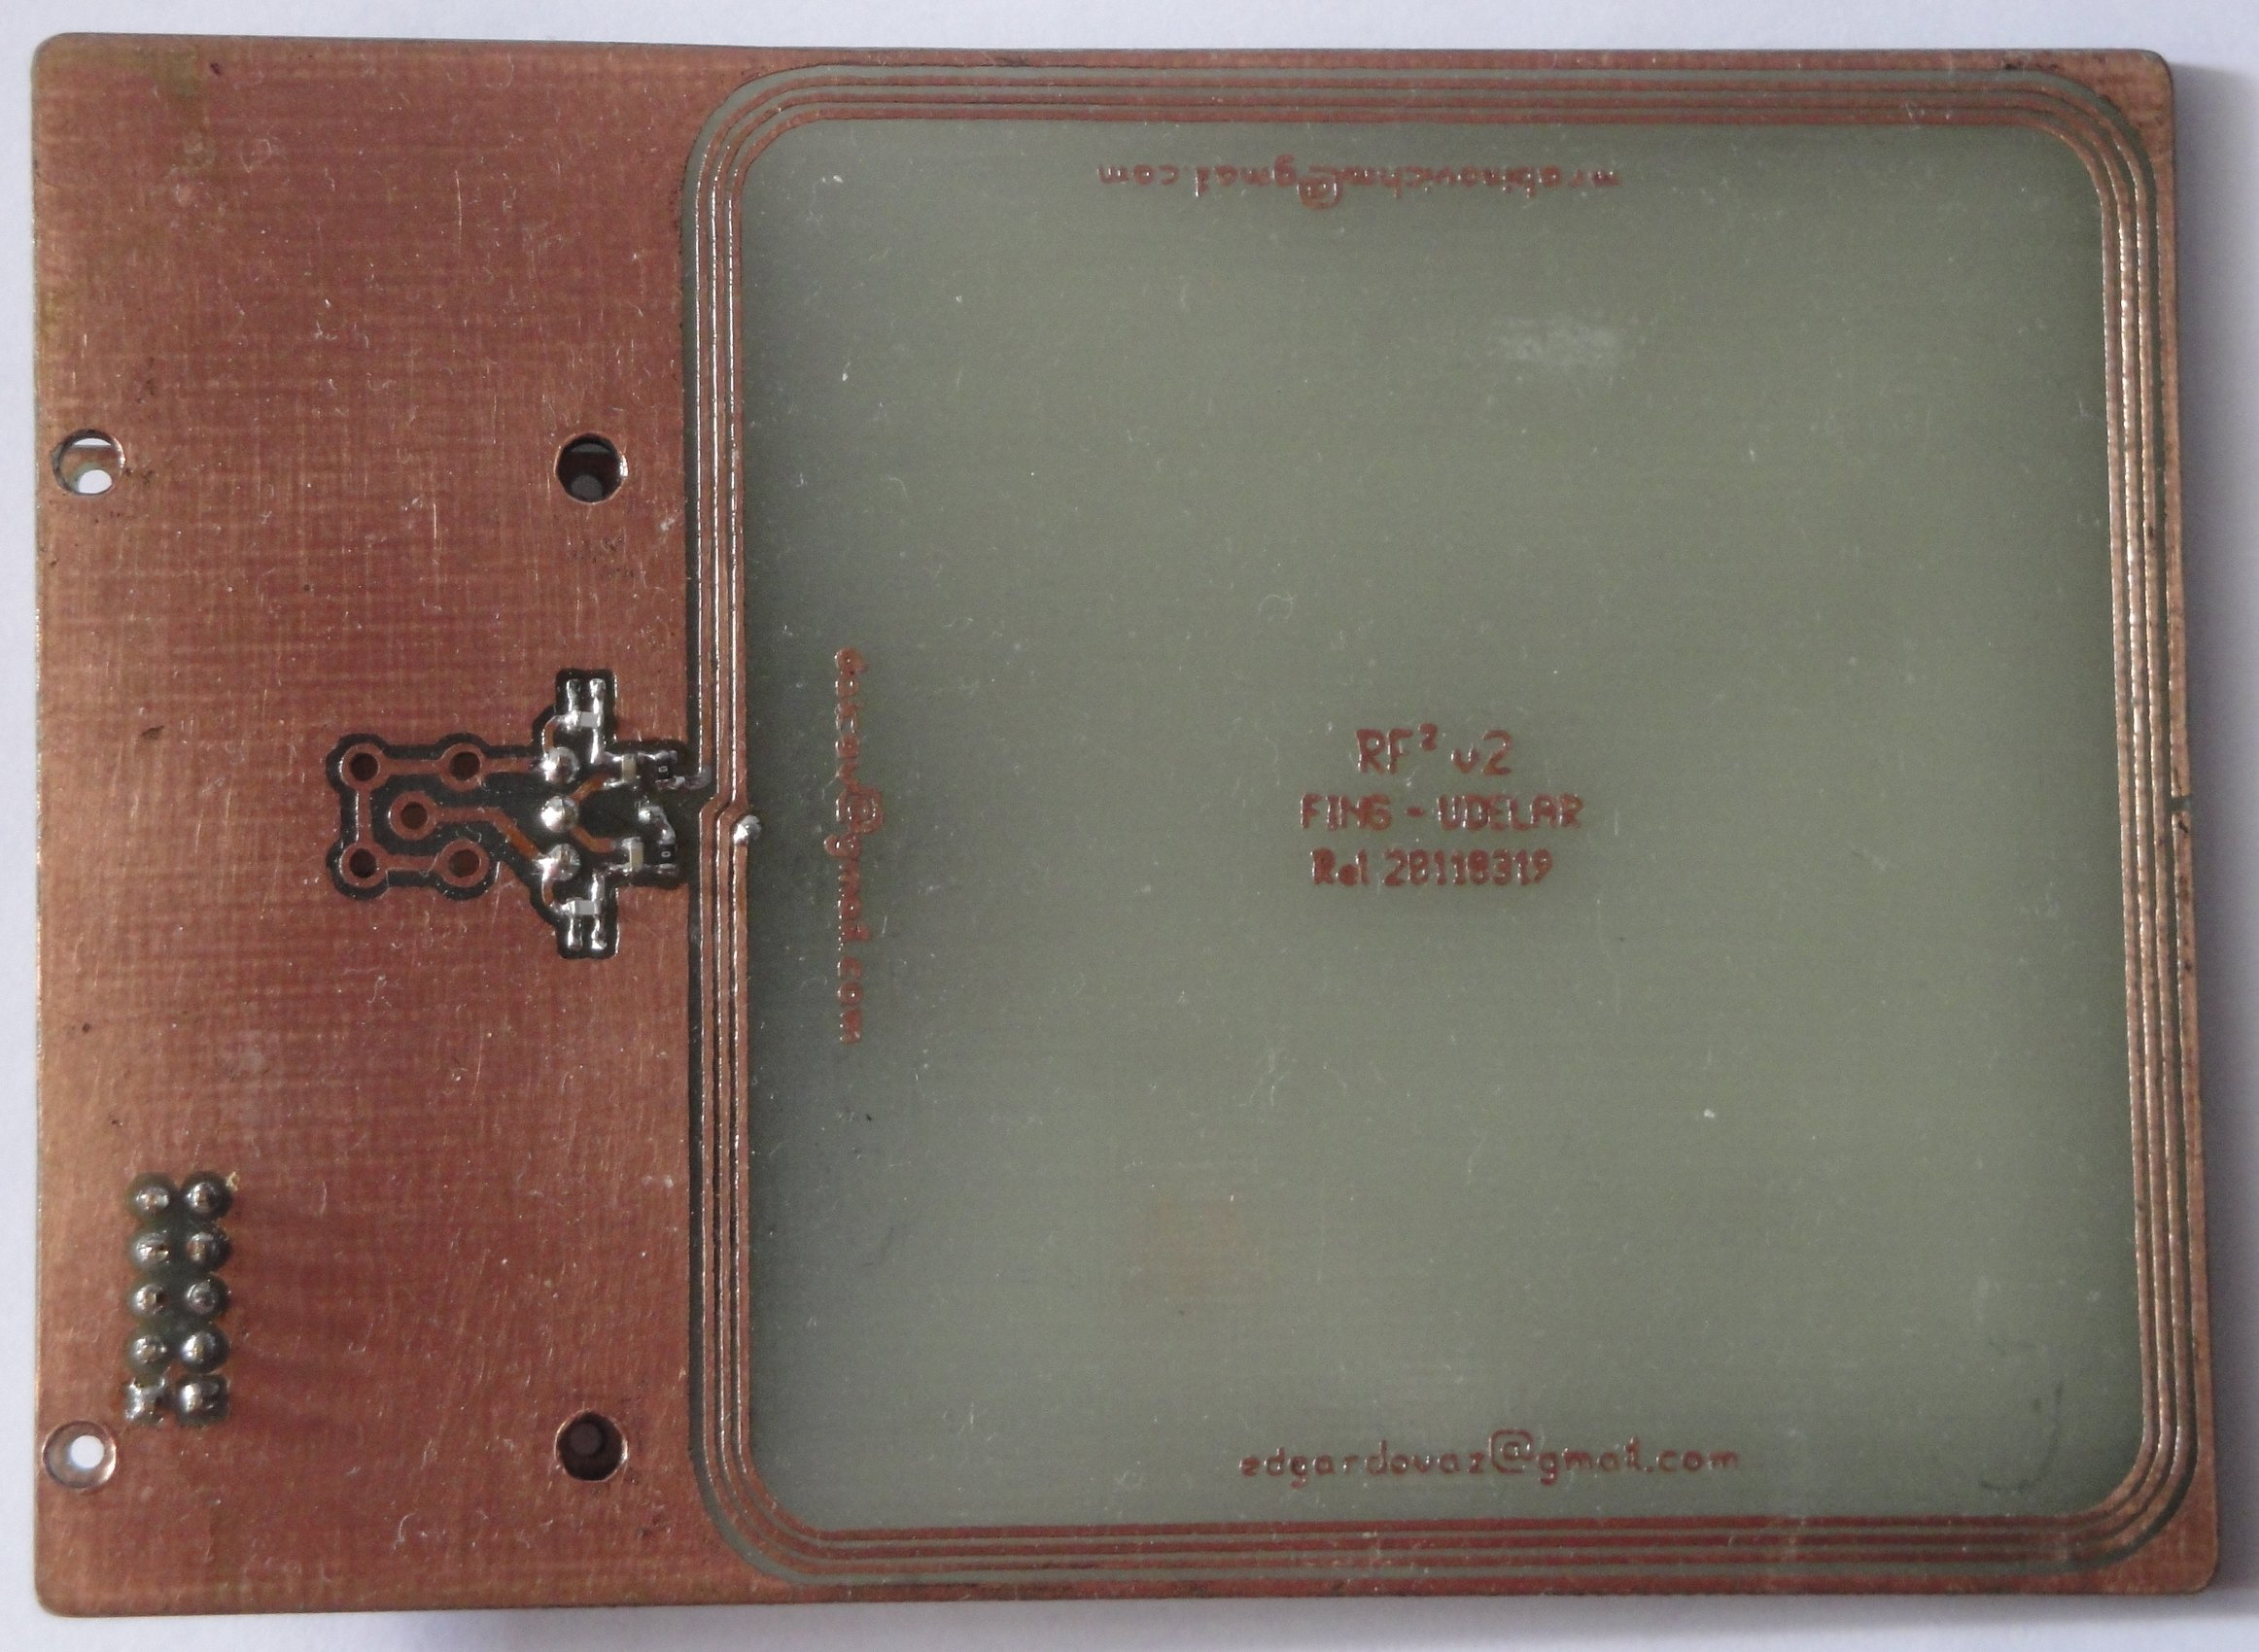
\includegraphics[scale=.08]{Imagenes/ant_f.jpg} } 
  \subfigure[Vista reversa del lector/escritor RFID]{\label{scuiB} 
  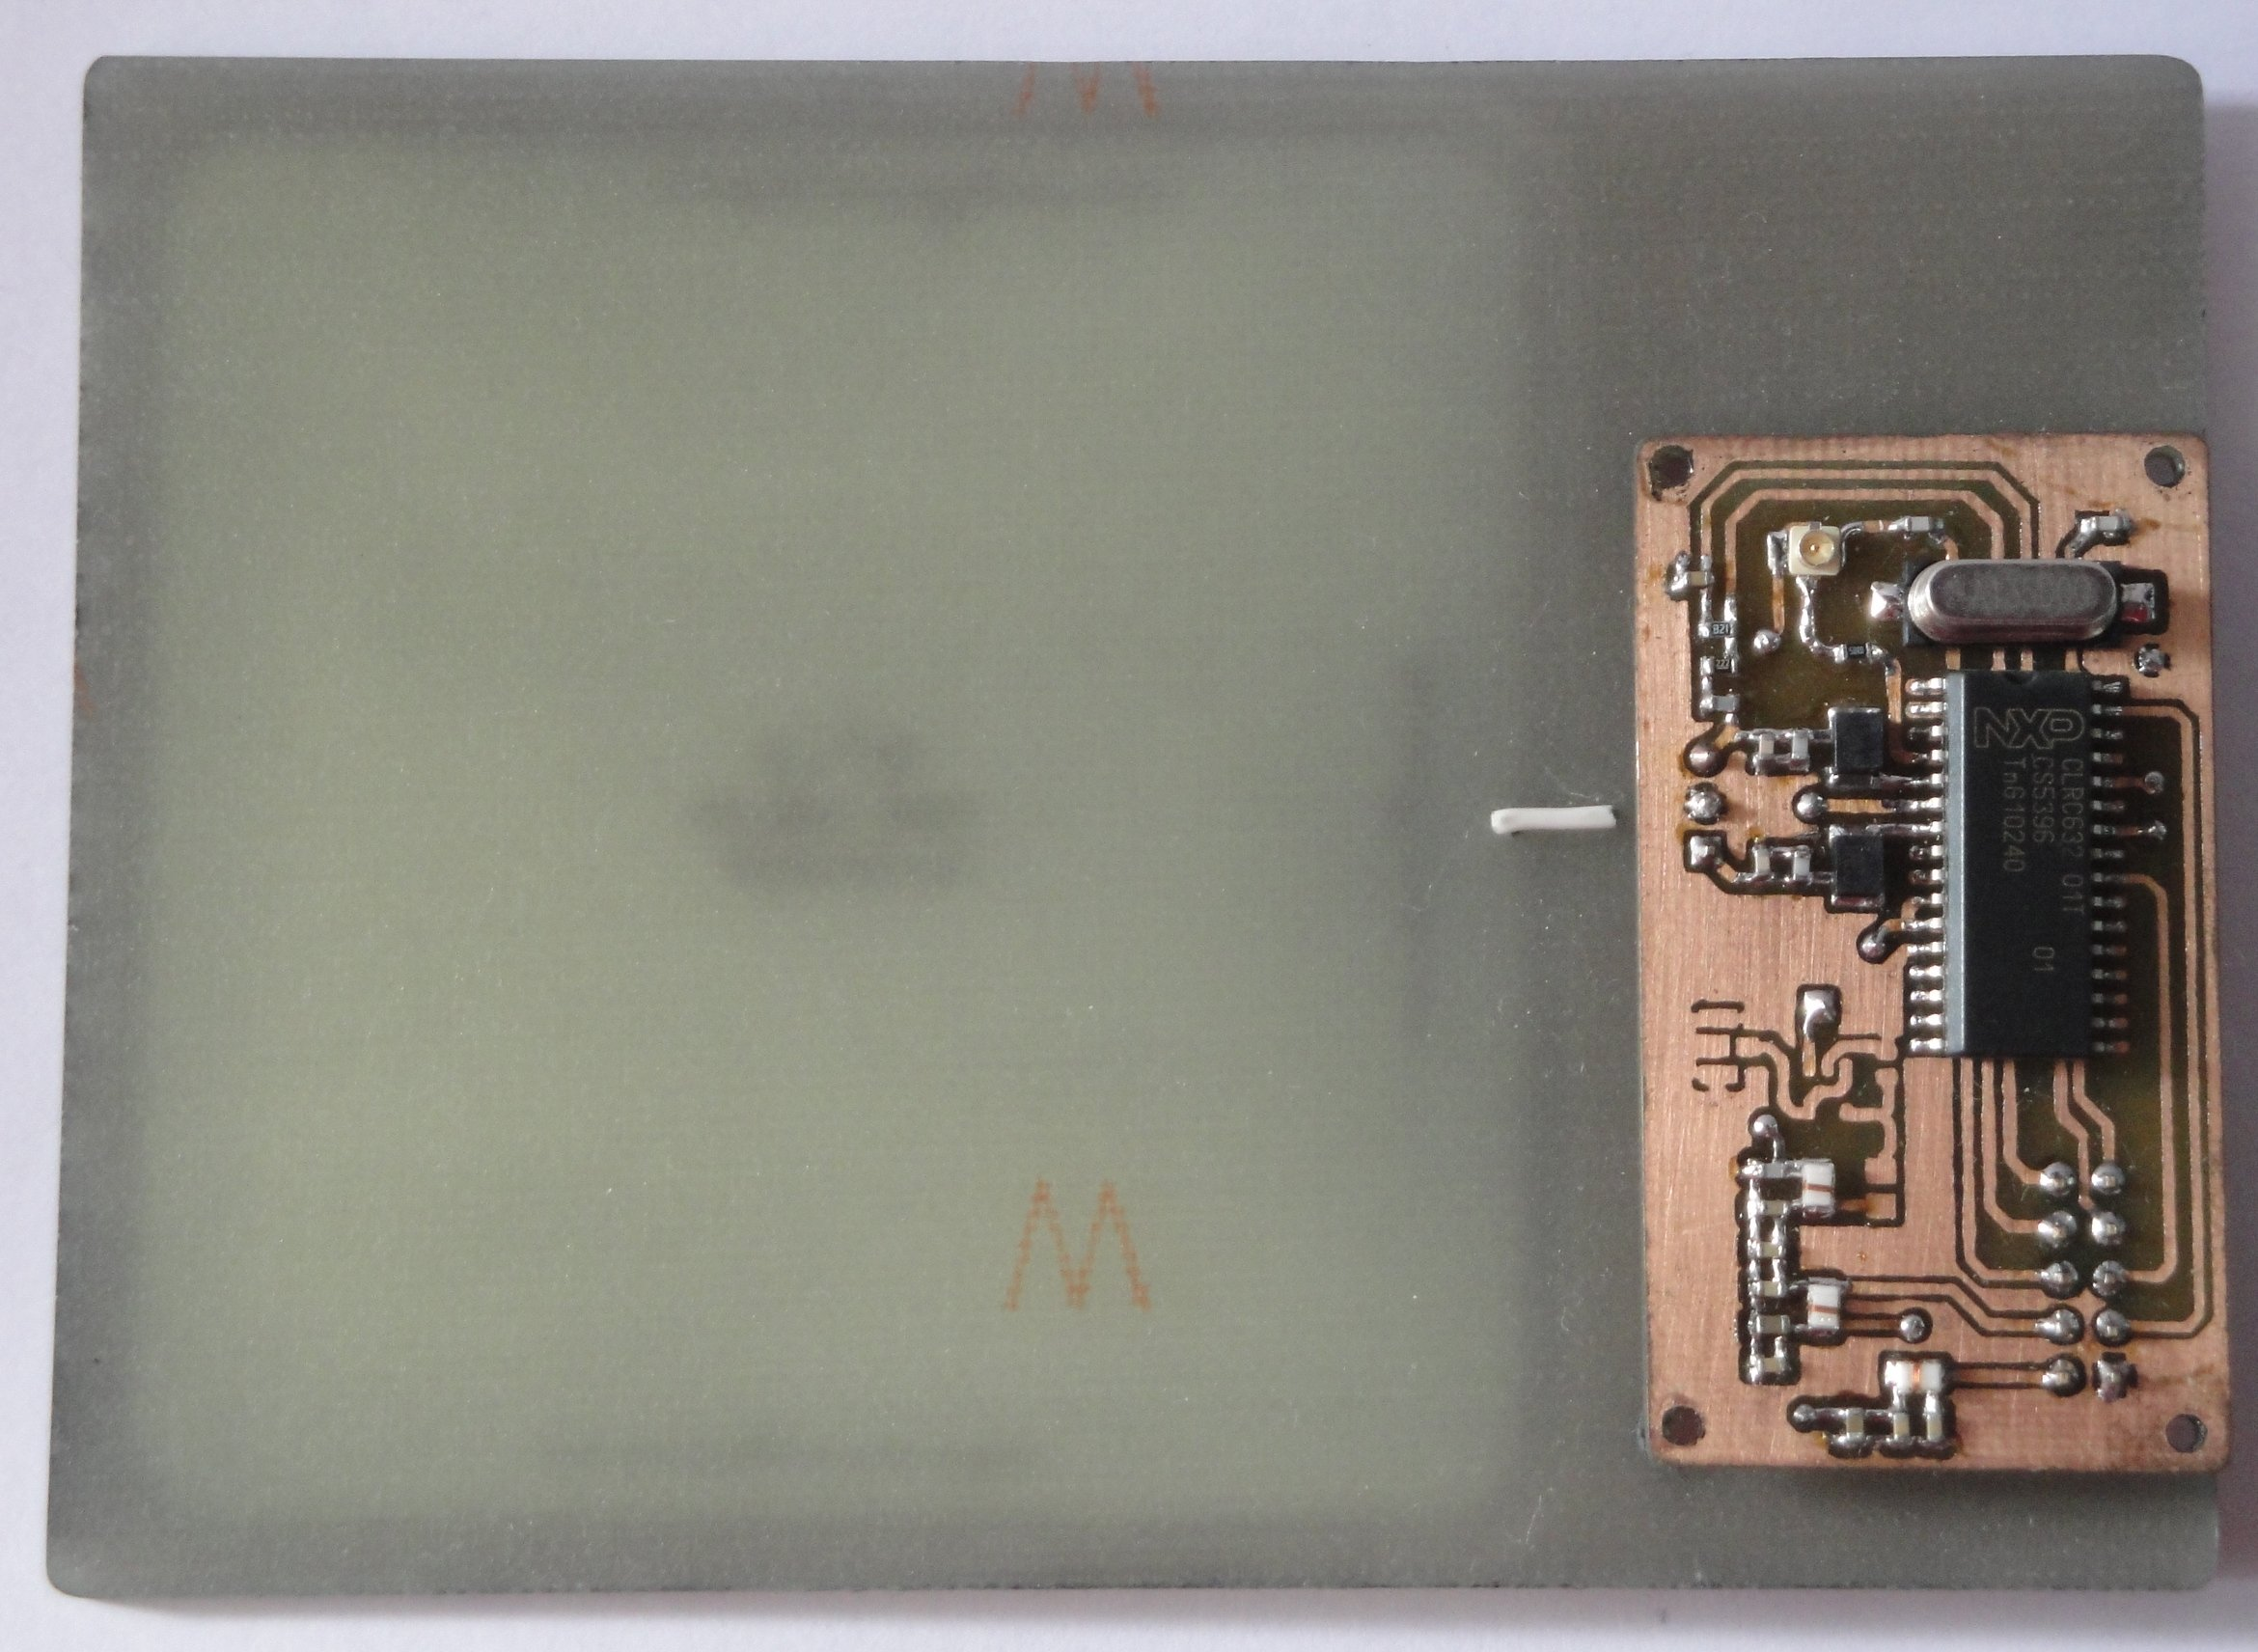
\includegraphics[scale=.08]{Imagenes/ant_b.jpg} }

  \caption{Vista anversa y reversa del lector/escritor RFID}\label{l/eRFID}
\end{figure}

\bigskip
Por detalles de esquemáticos y listas de componentes referirse al apéndice \ref{docHW}.

\newpage
\section{Funcionamiento de m\'odulos}

\subsection{SBC}
La SBC está formada por un SOC y memoria suficiente para ejecutar un sistema operativo GNU/Linux orientado a desarrollar sistemas embebidos. Sobre el sistema operativo se instalan los módulos y bibliotecas necesarias para hacer uso del hardware que contiene la SBC. En la aplicación se utilizará uno de sus puertos SPI para la comunicación con el lector/escritor de tarjetas RF, un puerto UART para la comunicación de datos con el lector de tarjetas de contacto y varias salidas GPIO para el control de la interfaz de usuario.

\subsection{VLT - Conversor de Voltajes}
El corazón de esta placa son los integrados TXB0108 \cite{HD_VLT} (ver hoja de datos en el apéndice \ref{HD}) que permiten la interconexión de dispositivos que operan en distintos niveles de tensión. Básicamente el integrado está constituído por dos puertos, puerto A y puerto B cada uno de 8 bits. El puerto A opera con la tensión de 1,8 Volt que permite ser conectado a la Beagleboard, el puerto B opera con la tensión de 3,3 Volt cuando se encuentra conectado al CL RC632, y de 5 Volt para los restantes periféricos.
Cada I/O de un puerto es sensible a los flancos de subida o bajada, trasladando estos cambios a la I/O correspondiente del puerto opuesto. 
Este integrado posee también una entrada de control para poner los puertos en estado de alta impedancia.
Una ventaja es que no poseen entrada de control de dirección de flujo de datos, de modo que se ahorran pines de control que no se tienen disponibles en la Beagleboard.
En la figura \ref{Fig:Celda_TXB0108} se puede observar como están constituídas cada una de las entradas/salidas del integrado.
Otra pieza que compone esta placa es el regulador de tensión LDO implementado a partir del integrado LM1117 \cite{LDO} (ver hoja de datos en el apéndice \ref{HD}), éste se utiliza para convertir la entrada de tensión de 5 Volt en una salida de tensión de 3,3 Volt y así poder alimentar el periférico correspondiente.

Por más detalles ver esquemático en la figura \ref{Fig:VLT}.

\bigskip
\bigskip
\begin{figure}[H]
\centering
  \begin{center}
  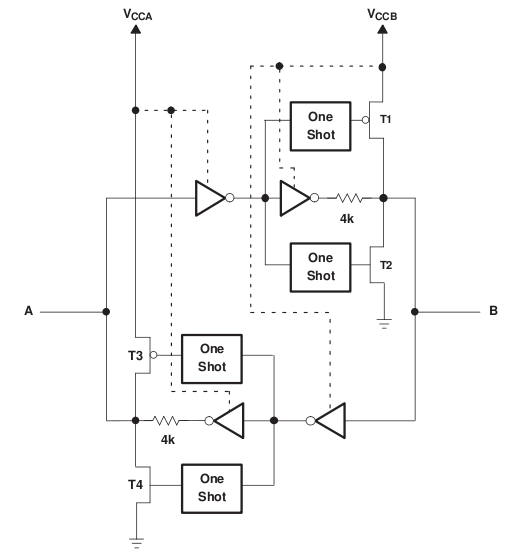
\includegraphics[scale=.3]{Imagenes/TXB0108.png} 
  \end{center}
  \caption{Arquitectura de una celda I/O del TXB0108}\label{Fig:Celda_TXB0108} 
\end{figure}


\subsection{SCUI - Lector de tarjetas de contacto e Interfaz de Usuario}

\leftline{\bf{Lector de tarjetas de contacto ISO7816}}

Es un lector muy simple de implementar, su construcción se basa en un conversor full a half duplex construido a partir de un circuito transistorizado trabajando en zona de corte y saturación. Los transistores empleados son el NPN 2N3904 (ver hoja de datos en el apéndice \ref{HD}) y el PNP 2N3906 (ver hoja de datos en el apéndice \ref{HD}) los cuales fueron seleccionados en base a su rápida característica de conmutación que es del orden de algunas decenas de nanosegundos. Dada la característica del circuito, es posible recibir el eco de la transmisión de datos generados por la SBC. 
Un elemento fundamental que compone el circuito del lector es el oscilador de frecuencia 3,579545 MHz, este valor no es antojadizo sino que permite generar la base de tiempo adecuada para la transmisión de datos entre la tarjeta y la SBC. Otras frecuencias de reloj fueron empleadas, como ser 4 MHz y 5 MHz, con resultados inciertos en la recepción de los datos, aún cuando sería posible usar estos valores según la referencia \cite{SCHb} para los parámetros obtenidos desde el ATR de la tarjeta. 
El circuito cuenta también con protección de descarga ESDA6V1W5 (ver hoja de datos en el apéndice \ref{HD}) para los contactos de la smart card.

Por más detalles ver esquemático en la figura \ref{Fig:SAM}.

\newpage
\leftline{\bf{Interfaz de usuario}}

El elemento a destacar es un display LCD16x2 que basa su funcionamiento en el controlador Hitachi HD44780 \cite{dpy} (ver hoja de datos en el apéndice \ref{HD}). La transferencia de datos hacia el display se hace a través de un puerto con 4/8 bits de datos y 3 bits de control. Debido a que no se cuenta con la cantidad de pines disponibles en la Beagleboard para operar en el modo de 8 bits, se empleó en su lugar el modo 4 bits del display. El bit de control RS indica si el byte a enviar por el puerto de datos es una palabra de control o un caracter ASCII a ser almacenado en la memoria interna del display. El bit R/W por su parte indica si se efectuará una lectura o una escritura de la memoria interna del display. Por último en el bit E se indica mediante flanco de bajada que se ejecute la operación indicada con los anteriores dos bits de control, previo a este flanco las señales en el puerto de datos deben permanecer fijas.
El display cuenta también con una entrada para calibrar el contraste del LCD, la calibración se realiza a partir de un divisor resistivo implementado con resistencias y un preset.
El backlight del display es accionado desde uno de los pines de la SBC a partir de un circuito transistorizado que opera en zona de corte/saturación.
Los restantes elementos que componen la interfaz de usuario son leds y buzzer que son accionados directamente desde los pines del puerto de expansión de la SBC.

Por más detalles ver esquemático en la figura \ref{Fig:UI}.

\subsection{Lector/Escritor RFID}
En el corazón del lector/escritor de tarjetas RFID, se encuentra el chip CL RC632 que forma parte de una familia de integrados empleados para la comunicación con tarjetas sin contacto, pertenecientes a la norma ISO14443 las cuales operan a la frecuencia 13,56 MHz.
El CL RC632 soporta todas las capas del esquema de comunicación que se establecen en la mencionada norma, incluyendo el algoritmo de seguridad (CRYPTO1) para autenticar las tarjetas Mifare Classic. En lo que sigue se describen algunas de las características principales del integrado.

Por más detalles ver esquemático en la figura \ref{Fig:RFID}.

\newpage
\leftline{\bf{Interfaz}}

Los comandos, bits de configuración y las banderas se acceden a través de la interfaz con un microprocesador. El puerto elegido para la comunicación desde la SBC es el SPI, aunque es posible la comunicación a través de su puerto paralelo. 

\bigskip
\leftline{\bf{Registros}}\label{Registros}

La configuración del chip se lleva a cabo a partir de un mapa de registros de control que se encuentra dividido en 8 páginas con 8 registros cada una. La manera de alcanzar estos registros es mediante el intercambio de página, mecanismo que puede ser deshabilitado mediante escritura de un “1” en el bit 7 del registro 0 en la página 0, logrando direccionamiento plano. La función de cada uno de sus registros puede ser observada en la hoja de datos del integrado \cite{RC632} (ver apéndice \ref{HD}).

\bigskip
\leftline{\bf{Memoria EEPROM}}

La memoria está dividida en 32 bloques con 16 bytes cada uno.
El contenido de memoria EEPROM en los bloques 1 y 2 (dirección 10hex a 2Fhex) se utilizan para configurar los registros del CL RC632 durante la fase de inicialización, de forma automática.
La configuración por defecto soporta la comunicación Mifare ISO 14443 A, aunque los usuarios pueden especificar la inicialización para I-Code1, ISO 15693 o ISO 14443 B, mediante los bloques de memoria 3 al 7.
Se reservan 384 bytes para almacenar las claves CRYPTO1 que son usadas para la autenticación con las tarjetas. El formato de una de estas claves puede verse en \cite{RC632} (ver apéndice \ref{HD}) y tiene una longitud de 12 bytes, por tanto es posible almacenar en memoria las 32 claves que posee una tarjeta.

\bigskip
\leftline{\bf{Buffer FIFO}}

El integrado contiente un buffer FIFO de 64 bytes para flujo de datos con un microprocesador.
La entrada y salida del buffer de datos está conectado con el registro FIFOData. Escribir en este registro almacena un byte en el buffer e incrementa el puntero de escritura del buffer. La lectura de este registro muestra el contenido del buffer e incrementa el puntero de lectura. La distancia entre el puntero de escritura y lectura se puede obtener mediante la lectura del registro FIFOLength, indicando así la cantidad de bytes que se llevan almacenados. Es posible observar y controlar el estado del buffer mediante varios registros, para evitar que se produzcan errores de comuncicación con el microprocesador.

\bigskip
\leftline{\bf{Interrupciones}}

El CL RC632 indica ciertos eventos estableciendo el bit IRQ en el registro \\
PrimaryStatus, y además, por la activación del pin IRQ. La señal en el pin IRQ se puede utilizar para interrumpir un micrprocesador. 
Las posibles fuentes de interrupción son: 

\begin{itemize}

\item Timer, a través de su bandera TimerIRq 
\item Transmisor, coprocesador CRC y memoria E2PROM, a través de su bandera TxIRq 
\item Receptor, a través de su bandera RxIRq 
\item Registro de comando, a través de su bandera IdleIRq 
\item Buffer FIFO, a través de sus banderas HiAlertIRq y LoAlertIRq 

\end{itemize}

El CL RC632 informa al microprocesador sobre el origen de una interrupción mediante el establecimiento del bit adecuado en el registro InterruptRq. La relevancia de cada bit de petición de interrupción como fuente de una interrupción puede ser enmascarada con el bit de habilitación de interrupciones en el registro InterruptEn. 
Si alguna bandera de solicitud de interrupción se establece en 1 (una solicitud de interrupción está pendiente) y la correspondiente bandera de habilitación de interrupción está en "1", la bandera de estado IRq en el registro PrimaryStatus se establece en 1. 
Por otra parte diferentes fuentes de interrupción pueden estar activas al mismo tiempo. Por lo tanto, se hace un OR con todos los bits de solicitud de interrupción, el resultado se envía a la bandera IRq y se conecta al pin IRQ. 
Los bits de petición de interrupciones están seteados de forma automática por las máquinas de estado internas del CL RC632. Adicionalmente, el microprocesador tiene acceso para setearlos o borrarlos. 
Una implementación especial de los registros InterruptRQ y InterruptEn permiten el cambio de un único bit de estado sin tocar el resto. 

\bigskip
Configuración del Pin IRQ:
El nivel lógico de la bandera de estado IRq es visible por el pin IRQ. Además, la señal en el pin puede ser controlada por los siguientes bits del registro IRQPinConfig 
\begin{itemize}
\item IRQInv: Si este bit es 0, la señal en el pin IRQ es igual al nivel lógico del bit IRq. 
Si es 1, la señal en el pin IRQ está invertida con respecto al bit IRq. 
\item IRQPushPull:  Si este bit es 1, el pin IRQ tiene características de una salida estándar 				   CMOS, de otra manera la salida es open drain y un resistor externo es necesario para alcanzar un nivel alto en este pin. 
\end{itemize}

Para poder hacer uso de lo descrito anteriormente se previó y reservó una entrada en el conector de expansión de la Beagleboard (ver figura \ref{Fig:VLT}), sin embargo el software empleado no hace uso del mecanismo de interrupciones sino que opera mediante polling.

\bigskip
\leftline{\bf{Transmisor, pines Tx1 y Tx2}}

La señal en Tx1 y Tx2 es la portadora, centrada en 13,56 MHz, modulada ASK 100\% con los datos a transmitir. Estos pines son conectados directamente a la antena para propagar la señal RF hacia las tarjetas RFID. La distancia de operación alcanzada es de hasta 10cm de longitud, dependiendo de la geometría de la antena, así como también adaptación de impedancia lograda, entre otros (ver \cite{MRICF} y \cite{RFIDPA} incluídas en el apéndice \ref{HD}).
Algunos registros del integrado permiten la configuración del transmisor, posibilitando entre otras cosas apagar la señal portadora en caso de ser necesario.

\bigskip
\leftline{\bf{Conjunto de comandos}}

El CL RC632 opera como una máquina de estado capaz de interpretar y ejecutar un conjunto de comandos pre establecidos. La ejecución de uno de ellos es posible escribiendo su código correspondiente en el “Registro de Comandos”, si fuera necesario el pasaje de parámetros, éstos se colocarán en el buffer FIFO mencionado antes. 
Una lista detallada de comandos junto con los parámetros necesarios es mostrada en la hoja de datos (ver apéndice \ref{HD}), entre ellos se pueden destacar los siguientes: Authent, Transceive, LoadKey.

\bigskip
\leftline{\bf{Antena RF}}

En lo que sigue se describen algunas de las partes que integran la antena RF que se conecta directamente a los pines Tx1 y Tx2 del integrado descrito antes.

\bigskip
\leftline{\bf{Filtro EMC}}

La frecuencia de la portadora de la señal transmitida se centra en 13,56 MHz, sin embargo se generan también armónicos de mayor frecuencia. Para cumplir con la regulación internacional EMC es que se agrega este filtro pasa bajos, cuya frecuencia de corte debe ubicarse en 14,4 MHz, o sea 13,56 MHz más 847,5 KHz para permitir el ancho de banda necesario que logre el baud rate requerido en la transmisión de los bits. 
En síntesis el filtro ayuda a mejorar la relación señal a ruido para la señal recibida y decrementa el sobretiro en los pulsos transmitidos mejorando la calidad de la señal transmitida.
Los valores propuestos para los componentes de este filtro se encuentran en las notas de aplicación \cite{MRICF}.

\bigskip
\leftline{\bf{Matching}}

Por su parte, el circuito de adaptación de impedancia permite que la antena resuene a la frecuencia deseada, en este caso 13,56 MHz. Los valores de los elementos que conforman este circuito deben ser estimados y sintonizados a partir del diseño del inductor de la antena.
El factor de calidad total de la antena debe ser tenido en cuenta para cumplir con los requerimientos establecidos en la norma ISO14443. 
El mecanismo para el cálculo de los elementos que foman este circuito se detallan en las notas de aplicación \cite{MRICF}.

\bigskip
\leftline{\bf{Inductor}}

El inductor de la antena es quien propaga el campo magnético para la transmisión de datos hacia las tarjetas. El diseño de la antena comienza a partir de este elemento.
El cálculo detallado del valor del inductor se encuentra en las notas de aplicación \cite{ACD}, aunque su costo y tiempo en la práctica son considerables; una estimación del valor de la inductancia puede verse en el apéndice \ref{anx_antena}, en el que se deben tener en cuenta los siguientes elementos: geometría de la antena, ancho y espesor del conductor del PCB, longitud de una espira, número de vueltas, etc.

\bigskip
\leftline{\bf{Receptor}} 

El circuito receptor de la antena se encuentra bien detallado en las notas de aplicación \cite{MRICF} y no fue necesario efectuar ningún cambio para lograr buenos resultados en este diseño particular. 

Por más detalles ver esquemático en la figura \ref{Fig:RFID2}.